% arara: pdflatex: { synctex: yes }
% arara: makeindex: { style: ctuthesis }
% arara: bibtex

% The class takes all the key=value arguments that \ctusetup does,
% and a couple more: draft and oneside
\documentclass[twoside]{ctuthesis}
\usepackage{float}
\usepackage{subcaption}
\usepackage{listings}
\usepackage[table,xcdraw]{xcolor}
\usepackage{longtable}
\usepackage{svg}
\usepackage{color,soul}
\usepackage{hyperref}
%\usepackage[backend=bibtex]{biblatex}

\clubpenalty 10000                      %kontrolovat sirotky
\widowpenalty 10000    

\usepackage[tableposition=top]{caption}
\usepackage{graphicx}

\newcommand{\diff}{\text{d}}
\newcommand{\mt}[1]{\text{#1}}


\definecolor{codegreen}{rgb}{0,0.6,0}
\definecolor{codegray}{rgb}{0.5,0.5,0.5}
\definecolor{codepurple}{rgb}{0.58,0,0.82}
\definecolor{backcolour}{HTML}{e5ecf6}

\renewcommand{\lstlistingname}{Ukázka kódu}% Listing -> Algorithm
\renewcommand{\lstlistlistingname}{Seznam ukázek kódu}% List of Listings -> List of Algorithms

\lstdefinestyle{mystyle}{
	backgroundcolor=\color{backcolour}, commentstyle=\color{codegreen},
	keywordstyle=\color{magenta},
	numberstyle=\tiny\color{codegray},
	stringstyle=\color{codepurple},
	basicstyle=\ttfamily\footnotesize,
	breakatwhitespace=false,         
	breaklines=true,                 
	captionpos=b,                    
	keepspaces=true,                 
	numbers=left,                    
	numbersep=5pt,                  
	showspaces=false,                
	showstringspaces=false,
	showtabs=false,                  
	tabsize=2,
	emph={int,char,double,float,unsigned,void,bool, uint8_t, uint16_t, int8_t, int16_t, grep},
	emphstyle={\color{blue}}
}
\lstset{style=mystyle}

\ctusetup{
	preprint = \ctuverlog,
%	mainlanguage = english,
%	titlelanguage = czech,
	mainlanguage = czech,
	otherlanguages = {slovak,english},
	title-czech = {Přenos telemetrických dat z meteorologického balónu},
	title-english = {Telemetric Data Transmission from Meteorological Balloon},
	subtitle-czech = {},
	subtitle-english = {},
	doctype = B,
	faculty = F3,
	department-czech = {Katedra elektromagnetického pole},
	department-english = {Department of electromagnetic field},
	author = {Jakub Dvořák},
	supervisor = {Ing. Tomáš Kořínek, Ph.D.},
	supervisor-address = {},
	supervisor-specialist = {},
	fieldofstudy-english = {},
	subfieldofstudy-english = {},
	fieldofstudy-czech = {},
	subfieldofstudy-czech = {},
	keywords-czech = {atmosféra, refrakce, meteorologická sonda, troposféra, útlum volného prostoru},
	keywords-english = {atmosphere, refraction, meteorological sonde, troposphere, free space loss},
	day = 20,
	month = 5,
	year = 2022,
	specification-file = {zav_prace.pdf},
%	front-specification = true,
%	front-list-of-figures = false,
%	front-list-of-tables = false,
%	monochrome = true,
%	layout-short = true,
}

\ctuprocess

\addto\ctucaptionsczech{%
	\def\supervisorname{Vedoucí}%
	\def\subfieldofstudyname{Studijní program}%
}

\ctutemplateset{maketitle twocolumn default}{
	\begin{twocolumnfrontmatterpage}
		\ctutemplate{twocolumn.thanks}
		\ctutemplate{twocolumn.declaration}
		\ctutemplate{twocolumn.abstract.in.titlelanguage}
		\ctutemplate{twocolumn.abstract.in.secondlanguage}
		\ctutemplate{twocolumn.tableofcontents}
		\ctutemplate{twocolumn.listoffigures}
	\end{twocolumnfrontmatterpage}
}

% Theorem declarations, this is the reasonable default, anybody can do what they wish.
% If you prefer theorems in italics rather than slanted, use \theoremstyle{plainit}
\theoremstyle{plain}
\newtheorem{theorem}{Theorem}[chapter]
\newtheorem{corollary}[theorem]{Corollary}
\newtheorem{lemma}[theorem]{Lemma}
\newtheorem{proposition}[theorem]{Proposition}

\theoremstyle{definition}
\newtheorem{definition}[theorem]{Definition}
\newtheorem{example}[theorem]{Example}
\newtheorem{conjecture}[theorem]{Conjecture}

\theoremstyle{note}
\newtheorem*{remark*}{Remark}
\newtheorem{remark}[theorem]{Remark}

\setlength{\parskip}{5ex plus 0.2ex minus 0.2ex}

% Abstract in Czech
\begin{abstract-czech}
	Tato práce se zabývá návrhem a realizací sondy, schopné měřit podmínky ve vyšších vrstvách zemské atmosféry. Naměřená data jsou zpracována a využita při tvorbě modelu šíření pro daný typ spoje. Práce obsahuje výběr stěžejních hardwarových komponent, návrh designu desek plošných spojů a stejně tak mechanickou zástavbu elektroniky. Dále se práce zabývá návrhem a realizací pozemní stanice, schopné přijímat data a formátovat je do zprávy pro anténní sledovač a realizací sledovacího softwaru na vykreslování trajektorie sondy v reálném čase. Práce poté zmiňuje jak způsoby testování elektroniky sondy, tak měření parametrů komponent, jež jsou součástí radiového spoje.
	
	V kapitole zaměřené na samotný experiment popisuje průběh experimentu a přípravu naměřených dat na další zpracování. Data jsou následně použita při tvorbě teoretického modelu šíření. 

\end{abstract-czech}

% Abstract in English
\begin{abstract-english}
	This thesis is focused on design and implementation of high altitude sonde capable of measuring conditions in upper atmosphere layers. Measured data are then processed and used in propagation model blablabla, nechám přeložit taťovi. 
\end{abstract-english}

% Acknowledgements / Poděkování
\begin{thanks}
Děkuji vedoucímu Tomášovi Kořínkovi za cenné rady a pomoc při realizaci práce. Děkuji Ing. Martinu Motlovi a Pavlu Žárskému za pomoc s vypouštěním sondy.

Dík také patří mé mamince za pomoc při hledání sondy a její nález. %Také děkuji za neustávající podporu v mých letech studentských. 
\end{thanks}

% Declaration / Prohlášení
\begin{declaration}
	Prohlašuji, že jsem tuto práci vypracoval samostatně s~použitím literárních pramenů a~informací, které cituji a~uvádím v~seznamu použité literatury a~zdrojů informací.

V Praze, \ctufield{day}.~\monthinlanguage{title}~\ctufield{year}
\end{declaration}

% Only for testing purposes
\listfiles
\usepackage[pagewise]{lineno}
\usepackage{lipsum,blindtext}
\usepackage{mathrsfs} % provides \mathscr used in the ridiculous examples

\begin{document}

\maketitle

\chapter{Úvod}
	\section{Cíl práce}
	%model šíření
	Tato práce je zaměřena na tvorbu modelu šíření radiového paprsku v atmosféře. Mezi prvky, ovlivňující kvalitu rádiového spoje, patří například ztráty volným prostorem, ale také troposférická refrakce - ohyb paprsku díky různým podmínkám v nižších vrstvách atmosféry.
	

	\section{Způsob řešení}
	%jak to budu řešit, stavba sondy, co bude měřit, měření na střeše s trackerem
	Pro měření podmínek ve troposféře bude zkonstruována meteorologická sonda vlastního návrhu, která bude schopna měřit veličiny, ovlivňující šíření radiového signálu. Mezi měřená data bude patřit teplota, relativní vlhkost a tlak. Přítomný GPS přijímač bude poskytovat zeměpisné souřadnice a nadmořskou výšku. Dále bude pozemním segmentem měřen výkon rádiového signálu a teoretický útlum bude porovnávaný s měřenými hodnotami. Uspořádání experimentu je vidět na obr. \ref{diagram:main}.

	\begin{figure}[hbtp]
		\centering
		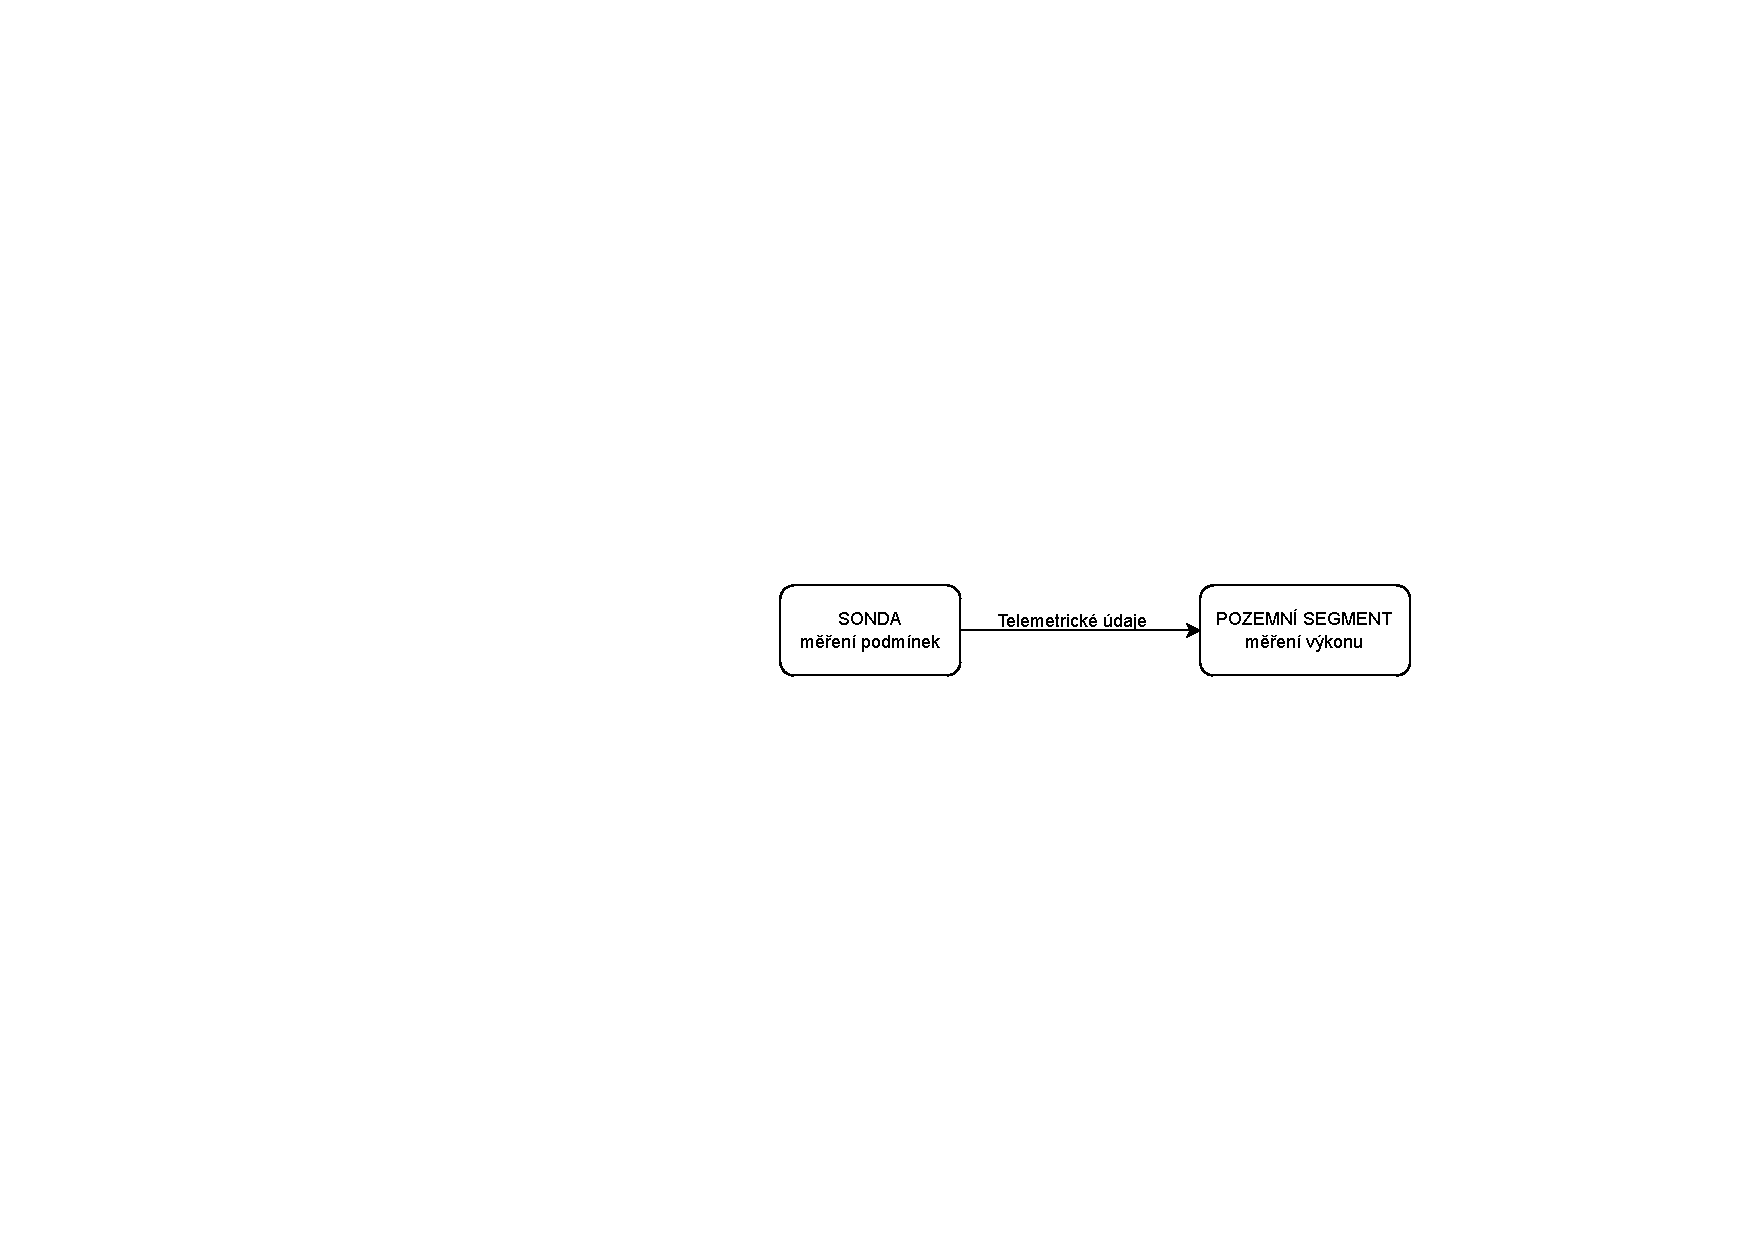
\includegraphics[width=.6\textwidth]{Figures/main_diagram.pdf}
		\caption{Hlavní uspořádání experimentu}
		\label{diagram:main}
	\end{figure}




	




























	

\chapter{Návrh experimentu}
	Následující kapitola popisuje teorii využívanou při návrhu experimentu a výběru senzorů. Nakonec popisuje samotný návrh experimentu, díky kterému je možné vytvořit matematický model přenosu radiového signálu a následné ověření modelu změřenými daty. 
	\section{Šíření vln ve troposféře}
		\subsection{Troposférická refrakce}
		Při průchodu vlny atmosférou Země je paprsek ovlivněn změnou prostředí, ve kterém se šíří. V závislosti na teplotě, tlaku a hustotě se mění i index lomu atmosféry, který má za následek refrakci - lom paprsku. Index lomu troposféry může nabývat hodnot mezi $n=1{,}000325$ při povrchu Země až $n=1{,}000110$ pro vrchní hranici troposféry~\cite{zaklady:sireni:vln}, nacházející se přibližně ve výšce 10~km \cite{web_tropo}.

		Pro přehlednost se zavádí tzv. refraktivita (\textit{refractivity N}), definována jako
		\begin{align}
			N = (n-1)\cdot 10^{-6}.
		\end{align}
		Jednotky refraktivity jsou tzv. \textit{N}-jednotky.

		Podle doporučení ITU-R P.453 \cite{ITU:refrac} lze pro frekvence do 100~GHz spočítat refraktivitu jako
		\begin{align}
			N = \frac{77.6}{T} \left(P + 4810\frac{e}{T}\right),
			\label{eq:tropo:refrac}
		\end{align}
		kde $T$ je absolutní hodnota v K, $p$ je atmosférický tlak v hPa a $e$ je tlak vodních par v hPa. Ten lze vypočíst pomocí hustoty vodních par z doporučení ITU-R 836 \cite{ITU:vapour}. Podle \cite{ITU:refrac} lze tlak vodních par vypočítat také podle relativní vlhkosti vzduchu $H$ jako
		\begin{align}
			e = \frac{H}{100}\,6{,}1121\,\mt{e}^{\frac{17{,}502t}{240{,}97 + t}},
			\label{eq:tropo:e}
		\end{align}
		kde $t$ je teplota v °C. Vztah platí v rozsahu teplot od -20 °C do 50 °C \cite{zaklady:sireni:vln}.

		Z rovnic \eqref{eq:tropo:refrac} a \eqref{eq:tropo:e} je patrné, že pro stanovení výškového profilu refraktivity je potřeba měřit teplotu, tlak a relativní vlhkost. 



		\subsection{Rádiový spoj}
		Před samotným návrhem elektroniky je potřeba navrhnout rádiovou linku a ověřit výkonovou bilanci rádiového spoje. Antény použité pro vysílání i příjem jsou kvadrifilární šroubovité antény s levotočivou polarizací. 

		Výkonová bilance spoje lze zapsat jako
		\begin{align}
			P_\mt{P} = P_\mt{V} + G_\mt{V} + G_\mt{P} + G_\mt{LNA} - FSL - L_\mt{kabel} - L_\mt{splitter},
			\label{eq:bilance}
		\end{align}
		Kde $G_\mt{V}$ a $G_\mt{P}$ jsou zisky antén, $P_\mt{V}$ je výkon vysílače měřený na vstupu antény, $G_\mt{LNA}$ zisk nízkošumového zesilovače, $FSL$ jsou ztráty volným prostorem, $L_\mt{kabel}$ ztráty kabelu a $L_\mt{splitter}$ ztráty děliče výkonu, rozdělující signál mezi spektrální analyzátor a přijímač radiového signálu.

		Ztráty volným byly spočteny podle \cite{zaklady:sireni:vln} jako
		\begin{align}
			L_\mt{FSL} = 32,4 + 20\mt{log}(f_\mt{MHz}) + 20\mt{log}(d_\mt{km}).
		\end{align}
		Jelikož jsou ztráty volným prostorem závislé na vzdálenosti, lze je vyjádřit pouze jako intervalem krajních hodnot. Místo vypuštění sondy, Praha - Libuš, je od buovy FEL v Dejvicích vzdálené 11,2~km. Maximální vzdálenost s ohledem na maximální výšku a predikci letu byla určena jako 50~km.

		Zisky resp. útlumy jednotlivých částí rádiové linky jsou zaneseny níže.
		\begin{align*}
			\begin{split}
				P_\mt{V} &= 22{,}3\mt{ dBm}\\
				G_\mt{V} &= 4{,}21\mt{ dBi}\\
				G_\mt{P} &= 4{,}21\mt{ dBi}\\
				G_\mt{LNA} &= 40 \mt{ dB}\\
				L_\mt{kabel} &= 2{,}5\mt{ dB}\\
				L_\mt{splitter} &= 3{,}6\mt{ dB}\\
				L_\mt{FSL} &= [112{,}16 .. 125{,}16]\mt{ dB}
			\end{split}
		\end{align*}

		Výsledný výkon očekávaný na vstupu spektránlího analyzátoru tedy bude po dosazení do \eqref{eq:bilance}:
		\begin{align}
			P_\mt{P} = 22{,}3 + 4{,}21 + 4{,}21 - [112{,}16~..~125{,}16] + 40 - 2{,}5 - 3{,}6\mt{ dBm}.
		\end{align}
		Hodnoty výkonu lze očekávat v rozmezí od $P_\mt{Pmax} = -48\mt{ dBm}$ do $P_\mt{Pmin} = -61\mt{ dBm}$.



		%budget link, co očekáváme za úrovně na základě budget linku












\chapter{Návrh systému}
V této kapitole se stanovují požadavky na systém a jsou specifikovány podmínky, ve kterých musí sonda fungovat a jaké parametry, jako např. hmotnost, musí sonda splňovat. Dále je vedena  diskuze o možných přístupech řešení elektroniky a ty jsou rozebírána z hlediska robustnosti a časové náročnosti. V této kapitole jsou také uvedeny nejpoužívanější způsoby sledování sondy, které jsou popsány a porovnány.

Schéma celé sestavy je zaneseno na obr. \ref{fig:sestava}.
\begin{figure}
	\centering
	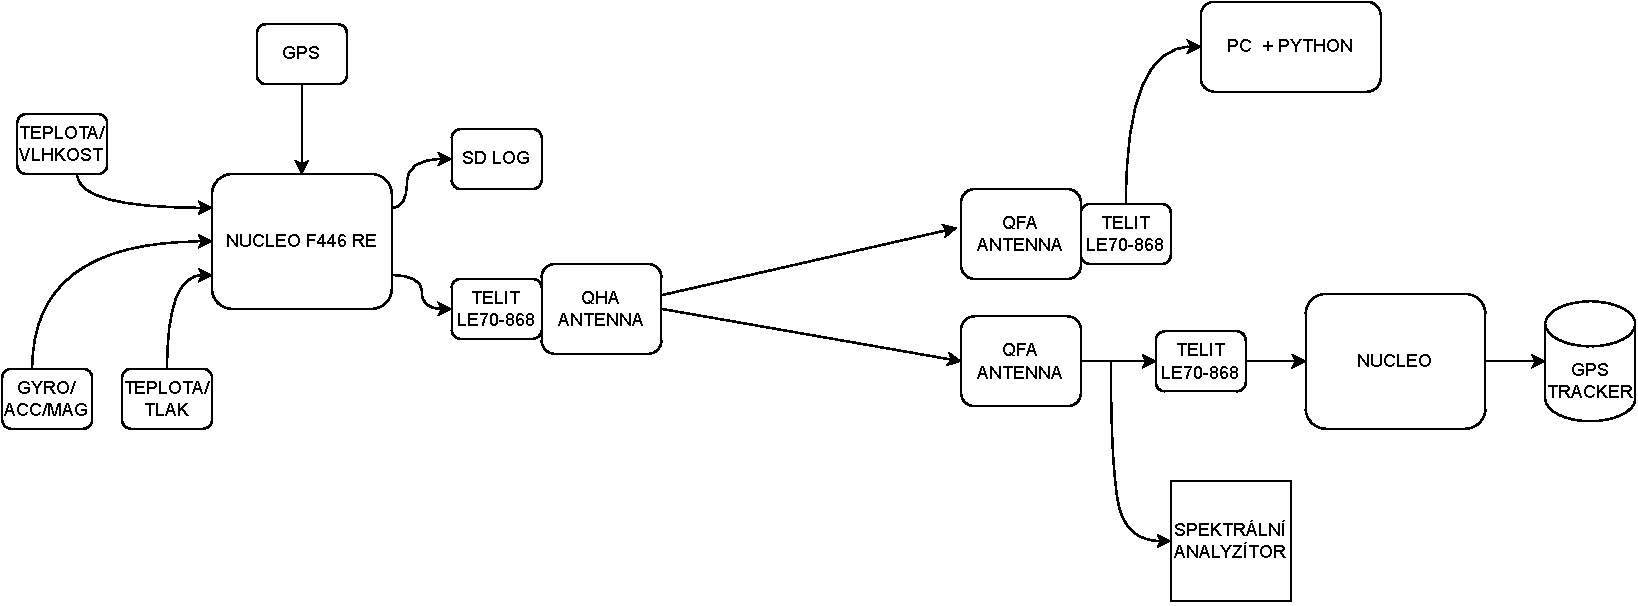
\includegraphics[width=\textwidth]{Figures/sonda_blokac.drawio.pdf}
	\caption{Blokové schéma sestavy}
	\label{fig:sestava:blokac}
\end{figure}

	\section{Požadavky}
	%co za data je potřeba pro model
	Hlavním požadavkem je posílání telemetrických údajů o poloze a ukládání zbylých naměřených dat na SD kartu umístěnou na palubě sondy. S ohledem na panující podmínky ve vyšších vrstvách zemské atmosféry musí být sonda schopna operovat za nízkého tlaku a teploty. Toto se vztahuje jak na mikročipy a senzory, tak na baterie, používané k napájení sondy. Další podmínkou je spolehlivé fungování v oblasti vysoké vlhkosti - oblačnosti a za deště. 

	Z důvodu dlouhé čekací doby na povolení vypuštění balónu, které vydává Úřad pro civilní letectví, je využito povolení, které má dlouhodobě sjednané ČHMÚ. Toto povolení se vztahuje na vypouštění volných balónů s užitečným zatížením do celkové hmotnosti 600~g. Denní sonda Vaisala RS41, kterou ČHMÚ posílá 3$\times$ denně, váží 84~g. Sonda vyvíjená v rámci této práce tedy musí splňovat požadavek na hmotnost do 516~g.

	Značná část GPS přijímačů je od výrobce zablokována pro použití ve výškách větších jak 10 km n. m. a je nutné zvolit přijímač, jehož maximální pracovní výška je alespoň 40~km.


	\section{Návrh systému}
		\subsection{Elektronika sondy}
		%součástky do -40, nízký tlak (bez elektrolytických kond.), dosah 40+ km

		V samotném návrhu elektroniky sondy byl možný zvolit jeden ze dvou přístupů. Níže práce popisuje výhody, nevýhody a potenciální rizika každé z nich. Dále zdůvodňuje přístup, který byl zvolen při řešení této práce.

		%snadné na vývoj a odladění, snadná změna zapojení pří psaní kódu
			\subsubsection{Využití vývojových modulů}
			V dnešní době existuje veliké množství mikročipů a MEMS čipů, které lze zakoupit ve formě modulů. Jedná se zpravidla o malé deky plošných spojů osazených konkrétními čipy s minimem potřebných součástek zajišťujících správné fungování. Zpravidla se jedná o blokovací kondenzátory umístěné v bezprostřední blízkosti čipů, poskytující elektrickou energii při rázovém odběru. Moduly mají vyvedené piny mikročipů na pinové lišty nacházející se zpravidla na okraji DPS. 

			V případě mikroprocesoru se jedná o vývojový kit Nucleo od firmy \textit{ST Microelectronics}. Kit se skládá z DPS s mikroprocesorem a minimem součástek, nutných pro správné fungování procesoru. Součástí desky je také zdroj pro napájení čipu a programátor, kterým lze do mikroprocesou nahrát firmware. Jednotlivé piny mikroprocesoru jsou vyvedeny na pinové lišty na kraji desky a slouží ke snadnému propojení s moduly. 

			Výhodou tohoto řešení ve fázi vývoje je snadná záměna zapojení modulů a rychlé odstranění chyb způsobené chybným výběrem komunikačních pinů mikroprocesoru.

			Nevýhoda tohoto řešení je malá robustnost zapojení. Komunikační cesty mezi mikroprocesorem a senzory jsou zbytečné dlouhé, jelikož jsou podřízeny umístění pinů na pinových lištách. Další nevýhodou je nemožnost ovlivnit umístění blokovacích kondenzátorů u mikroprocesoru a nebo zvýšení jejich počtu. Vývojový kit Nucelo není tvořen s ohledem na malé rozměry a velikost DPS tohoto kitu ovlivňuje celkovou velikost a hmotnost sondy.

			\subsubsection{Samostatné senzory}
			Druhá cesta, kterou je možná se vydat při vývoji elektroniky v sondě je samostatná deska, která obsahuje jednotlivé mikročipy bez jejich modulů a separátních DPS. Díky tomu je možné minimalizovat vzdálenost mezi mikroprocesorem a senzory a zvýšit robustnost napájení čipů. Celková velikost desky je poté dána především schopnostmi návrháře. 

			Toto řešení je časové náročnější, než první zmíněné a v případě způsobené chyby se špatně odstraňují chyby. V případě zničení, nebo nefunkčnosti nějaké elektronické součástky je nutné její odpájení z desky, což může ohrozit komponenty v okolí. V případě modulů lze vyměnit modul samotný.

			Při řešení této práce byla zvolena cesta modulů. Důvodem bylo malé množství času neumožňující případné zdlouhavé odlaďování zapojení a také nedostatek součástek samotných. V tomto případě byly dostupnější senzory ve formě modulů a mikroprocesor ve formě vývojového kitu. 

			
		\subsection{Sledování sondy}
		Sledování sondy lze realizovat několika způsoby. Níže jsou popsány nejčastější z nich a jsou diskutovány výhody, nevýhody a možná rizika.

				\subsubsection{GSM tracker}
				Amatéry často využívána, nicméně nedoporučovaná metoda \cite{web_sledovani} je zasílání dat skrze mobilní sítě. GSM sítě, přes které se data posílají, jsou určena pro telefony v okolí země a ve vyšších výškách může dojít k výpadku signálu. Velké množství sond také přistane v~neobydlených a~odlehlých oblastech, ve kterých nemusí být dostatečný signál pro přenos dat.


				\subsubsection{APRS}
				APRS (\textit{\textbf{A}utomatic \textbf{P}acket \textbf{R}eporting \textbf{S}ystem}) je radioamatéry často využívaný způsob sledování sondy, jelikož jde o~způsob levný a spolehlivý a~mnoho radioamatérů má vlastní vybavení pro posílání dat přes APRS. Základem je APRS vysílač, který lze koupit, nebo postavit. GPS data, spolu například s~teplotou a~tlakem, jsou následně takto vysílána a~přijímána amatérskými rádii~\cite{web_sledovani}. Data se poté buď pošlou dál, nebo se nahrají na internetovou stránku k tomuto účelu zřízenou, odkud je může každý sledovat.\footnote{\url{aprs.fi}}
				Nevýhodou APRS sledovače je bohužel fakt, že pokud sonda přistane v~neobydlené a~odlehlé oblasti, kde nejsou žádné amatérské rádiové stanice, není možno data odeslat. Proto je APRS sledovač vhodný pouze jako záloha, nebo doplnění, není dobré na něj spoléhat se stoprocentní jistotou. Pokud se vysílači nepovede vyslat souřadnice místa dopadu, můžeme přesto APRS vysílač najít pomocí radiového přijímače, naladěného na vysílací frekvenci, a~směrové antény. Další nevýhoda je potřebná licence pro vysílání na frekvenci 144,8~MHz, na které probíhá APRS \cite{web_ctu}.


				\subsubsection{Satelitní sledovač}
				Další způsob je využité satelitního sledovače. Jedná se zpravidla o zařízení na sledování majetku v případě odcizení. Získaná data o~poloze se posílají přes síť satelitů na nízké oběžné dráze Země. Využívána je služba \textit{Globalstar}, jež se specializuje na provoz satelitních telefonů. Ze satelitů jsou následně data poslána na speciální internetovou stránku, kde jsou přístupná například z~počítače, nebo mobilní aplikace. Pozice lze také zaslat přes SMS bránu, jako zprávu na mobilní telefon. Výhodou je širší pokrytí oproti GSM síti. 

				Toto řešení má nicméně i~své nevýhody. GPS čip ve sledovači je omezený do maximální výšky 6\,500\,m\,n.\,m.~\cite{web_spot}. Kvůli tomu nastane po dosažení takové výšky tzv. blackout, kdy GPS čip přestane reagovat. Po následném sestupu sondy pod hladinu 6\,500\,m\,n.\,m. se GPS čip opět připojí a~sledovač opět začne fungovat. Další z~problémů je fakt, že sledovač musí mít GPS anténu neustále nasměrovanou k~obloze, tudíž, pokud se při dopadu sonda nějak překlopí, není možné zaměřit její pozici.

				\subsubsection{Přímé posílání GPS dat}
				Pro tuto práci je implementačně nejjednodušším řešením přímé posílání GPS dat. S ohledem na zadání je nutné v rámci práce telemetrická data o poloze ze sondy posílat a tedy tyto informace lze využít k samotné lokalizaci a následnému nalezení sondy. Rizikem je dopad do oblasti, kde se omezí dosah telemetrického signálu. Např. do hustého lesa, nebo do zástavby.

				S ohledem na hmotnost, kterou by předešlá řešení přidala k celkové hmotnosti, bylo zvoleno tohoto způsobu sledování.

				\subsubsection{Zjištění pozice sondy ČHMÚ}
				Jak již bylo zmíněno, sonda ČHMÚ je při letu zavěšena pod vyvíjenou sondou. Data vysílaná sondou ČHMÚ jsou přijímána a dekódována v místě vypuštění, ale také jsou zachytávána amatérskými rádii a informace o poloze jsou sdílena na internetu. Tento způsob je spolehlivý, jelikož vysílací část je komerčně prodávaná a určena pro profesionální použití. Přijímacích stanic je velké množství a tedy je vysoká pravděpodobnost, že budou data ze sondy zachycena. 

				Nevýhodou je, že sonda ČHMÚ není přímou součástí vyvíjené sondy a tedy může dojít k odtržení. Tento způsob sledování je tedy brán jako záloha.


		
		\subsection{Firmware sondy}
		Firmware pro mikroprocesor v sondě zajišťuje inicializaci senzorů, správné čtení dat ze senzorů, jejich zpracování. Dále je nutné načítání data z GPS modulu a jejich rozdělení na dané zprávy a bloky informací využívaných pro určení pozice v prostoru. Všechny získané informace je poté nutno sešít do zprávy poslané telemetrií na zem a uložit na externí paměť. 

		Nutnou součástí firmwaru je také ošetření chybových stavů a možných errorů, vyvolaných chybným čtením dat a nebo fyzickými podmínkami prostředí.

		\subsection{Mechanická zástavba}
		Mechanická zástavba celé sondy musí splňovat požadavky pracovníků ČHMÚ, aby nedošlo k poničeni balónu a způsobení škod při dopadu na zem. Jelikož je sonda Vaisala RS41 pověšena pod sondu vznikající v rámci této práce, je nutné zajistit robustnost a zamezit odpojení sondy Vaisala, nebo rozpadu vyvíjené sondy.



		\subsection{Pozemní stanice}
		\label{sec:navrh:pozemni_stanice}
		Firmware pro mikroprocesor v pozemní stanici zodpovídá za správné dekódování přijatých telemetrických údajů. Firmware musí určit, která data jsou validní. Přijatá data je poté nutno zformátovat do zprávy určené pro anténní tracker, umístěný na střeše budovy FEL. Firmware musí být odolný vůči náhodným chybám způsobených přenosem na velkou vzdálenost. Příjem i posílání dat probíhá přes sériovou linku. 

		Elektronika pozemní stanice není vystavena extrémním podmínkám a není nutné řešit její odolnost vůči vnějším vlivům. 


		\subsection{Software pro zobrazení telemetrických údajů}
		Software určený pro příjem dat na počítači umístěném v automobilu jedoucí ve směru dopadu sondy. Software musí určit validní data a vyznačit GPS pozici sondy na mapě. Další funkcí softwaru je výpis souřadnic, výšky a rychlosti sondy a teploty okolí sondy. Data jdoucí do programu jsou posílána přes sériovou linkou z přijímače signálu vysílaného sondou. 




\chapter{Realizace systému}
Tato kapitola se zabývá samotnou realizací sondy. V textu jsou uvedeny jednotlivé moduly zodpovídající za měření dat a jsou popsány motivace jejich výběru. Dále text rozebírá dílčí části firmwaru sondy a způsob, jakým byly řešeny problémy, které nastaly vinou nestandardních podmínek. Popisuje jak vysílací část - sondu, tak přijímací části; pozemní stanici, která formátovala data do zprávy čitelné anténním trackerem a přijímací software na zobrazení pozice na mapě. 

	\section{Elektronika sondy}
		\subsubsection{Použité komponenty}
		Níže jsou zmíněny druhy senzorů, které jsou nutné pro měření podmínek v troposféře, které ovlivňují přenos radiového signálu. Jak již bylo zmíněno, senzory musí být schopny měřit veličiny v rozsahu hodnot, které panují ve troposféře. Velký výběr modulů s mnohými senzory a dalšími elektrickými součástkami nabízí firma \textit{Microelektronika}. Jená se o produky využívané pro výuku a rychlý vývoj. Výhodou je jejich sjednocený pinout a stejné rozměry konektoru (pinové lišty). Další důvod pro vyběr modulů od tohoto výrobce byla již jejch dostupnost na katedře elektromagnetického polel

			\subsubsection{GPS modul}
			GPS moduly jsou zpravidla omezeny dvěma parametry. Maximální nadmořsou výškou 18~km a maximální rychlostí 515~m/s vůči zemi https://www.ecfr.gov/current/title-22/part-121. Někteří výrobci GPS modulů berou tato omezení v konjunkci, kdy pro zablokování modulu musí platit obě podmínky, někteří výrobci uvažují  disjunkci, kdy stačí, aby nastala jedna z pomínek a modul přestane dávat validní data. Modul, který byl vybrán je u-blox SAM-M8Q. Podle dokumentace GPS modulu (\url{https://www.u-blox.com/sites/default/files/SAM-M8Q_DataSheet_%28UBX-16012619%29.pdf}) je maximální výška 50~km a maximální rychlost 500~m/s. V případě letu balónu nebude splněna ani jedna z podmínek. Tento GPS modul je součástí vývojového modulu GNSS 4 Click od firmy \textit{Microelektronika}.

			U-Blox moduly nabízí široké množství pracovních módů podle charakter použití. Pro běžné použití se využívá mód \textit{Portable}. Jedná se o kompromis mezi rozsahem a přesností určení pozice. Další módy jsou zobrazeny v tabulce \ref{tab:ublox:modes}. V případě sondy byl zvolen mód Airborne \textless{}1g. Při letu sondy není očekáváno zrychlení přesahující 1~g a rychlosti nad 100~m/s (360~km/h). 
			\begin{table}[]
				\centering
				\caption{Módy GPS přijímačů u-blox}
				\label{tab:ublox:modes}
				\begin{tabular}{|l|c|c|c|c|}
					\hline
					Platform &
					Max Altitude (m) &
					\begin{tabular}[c]{@{}c@{}}MAX Horizontal\\ Velocity (m/s)\end{tabular} &
					\begin{tabular}[c]{@{}c@{}}MAX Vertical\\ Velocity (m/s)\end{tabular} &
					\begin{tabular}[c]{@{}c@{}}Max Position \\ Deviation\end{tabular} \\\hline
					Portable               	& 12000 & 310 & 50  & Medium \\\hline
					Stationary             	& 9000  & 10  & 6   & Small  \\\hline
					Pedestrian             	& 9000  & 30  & 20  & Small  \\\hline
					Automotive             	& 6000  & 84  & 15  & Medium \\\hline
					At sea                 	& 500   & 25  & 5   & Medium \\\hline
					Airborne \textless{}1g 	& 50000 & 100 & 100 & Large  \\\hline
					Airborne \textless{}2g 	& 50000 & 250 & 100 & Large  \\\hline
					Airborne \textless{}4g 	& 50000 & 500 & 100 & Large  \\\hline
					\end{tabular}
				\end{table}
			


			
			\subsubsection{Teplotní a tlakový senzor}
			Podle (\url{https://www.sensorsone.com/altitude-pressure-units-conversion/}) se tlak ve výšce 30~km pohybuje kolem hodnoty 10~mbar. S ohledem na očekávané rozsahy měřeného tlaku a teploty byl vybrán senzor MS5607 od firmy \textit{TE Connectivity}. Rozsahy měřitelných hodnot jsou zaneseny v tabulce \ref{tab:ms:range}. Teplotní a tlakový senzor je součástí modulu od firmy \textit{Parallax}. Výrobce na stránkách produktu \url{https://www.parallax.com/product/altimeter-module-ms5607/} uvádí, že senzor byl úspěšně testován ve výšce 36~km.
			
			\begin{table}[]
				\begin{tabular}{|l|lll|l|}
				\hline
				Pressure   & \multicolumn{1}{l|}{Min}  & \multicolumn{1}{l|}{Typ} & Max  & Unit \\ \hline
				Range      & \multicolumn{1}{l|}{10}   & \multicolumn{1}{l|}{}    & 1200 & mbar \\ \hline
				Range      & \multicolumn{1}{l|}{-40}  & \multicolumn{1}{l|}{}    & 85   & °C   \\ \hline
				Resolution & \multicolumn{3}{c|}{\textless{}0.01}                        & °C   \\ \hline
				Accuracy   & \multicolumn{1}{l|}{-0.8} & \multicolumn{1}{l|}{}    & 0.8  & °C   \\ \hline
				\end{tabular}
				\caption{Rozsah senzoru MS5607, převzato z \url{https://www.parallax.com/package/altimeter-module-ms5607-datasheet})}
				\label{tab:ms:range}
			\end{table}

			


			
			\subsubsection{Vlhkostní senzor}
			Vlhkostní senzor byl zvolen AM2320, který je součástí modulu DHT22 Click od firmy \textit{Microelektronika}. Senzor je schopen měřit v rozsahu od -40 do 80~°C a 0 až 100~\% relativní vlhkosti (\url{https://cdn-shop.adafruit.com/product-files/3721/AM2320.pdf}). 



			
			\subsubsection{Senzor orientace}
			Pro zjištění orientace bylo použito senzoru MPU9250, který je součástí modulu 9DOF Click. Jedná se o gyroskop Senzor resp. modul byl vybrán, jelikož byl již dříve používán na jiných projektech a byl ihned dostupný. Díky tomu bylo ihned možné přejít ke psaní ovladače pro vyčítání dat a jeho implementaci do systému. Senzor také splňuje rozsah pracovních teplot a lze tedy využít v podmínkách, které při letu nastanou (\url{https://invensense.tdk.com/wp-content/uploads/2015/02/PS-MPU-9250A-01-v1.1.pdf}).  
			

			\subsubsection{Radiový vysílač/přijímač}
			Pro přenos dat vyl využit readiový vysílač Telit LE70 - 868. Jdná se o téměř \textit{\&play} zařízení. Data jsou do modulu posílána přes sériovou linku UART, odkud jsou následně přeposlána dál. Modul pracuje v režimu Half Diplex a tedy stejný typ modulu lze využít na příjem i vysílání dat bez nutnosti měnit nastavení. 


		
		

		
		\subsection{DPS pro připojení modulů}
		%Navrženy shieldy, nakresleny modely. Spínaný zdroj + LDO, ochrany vstupů, volné GPIO na rozšíření
		Ve vývojové fázi práce byly moduly zapojeny skrze nepájivé pole a propojeny propojovacími kabely s piny Nucleo desky. Moduly byly postupně přidávány souběžně s vývojem softwaru. Po odladění komunikace se všemi použitými moduly byly vytvořeny dvě redukční DPS na propojení Nucleo kitu a modulů. Moduly jsou vyobrazeny na obr. \ref{fig:shield:top} a \ref{fig:shield:bot}. 

		\begin{figure}[hbtp]
			\centering
			\begin{subfigure}{0.3\textwidth}
				\centering
				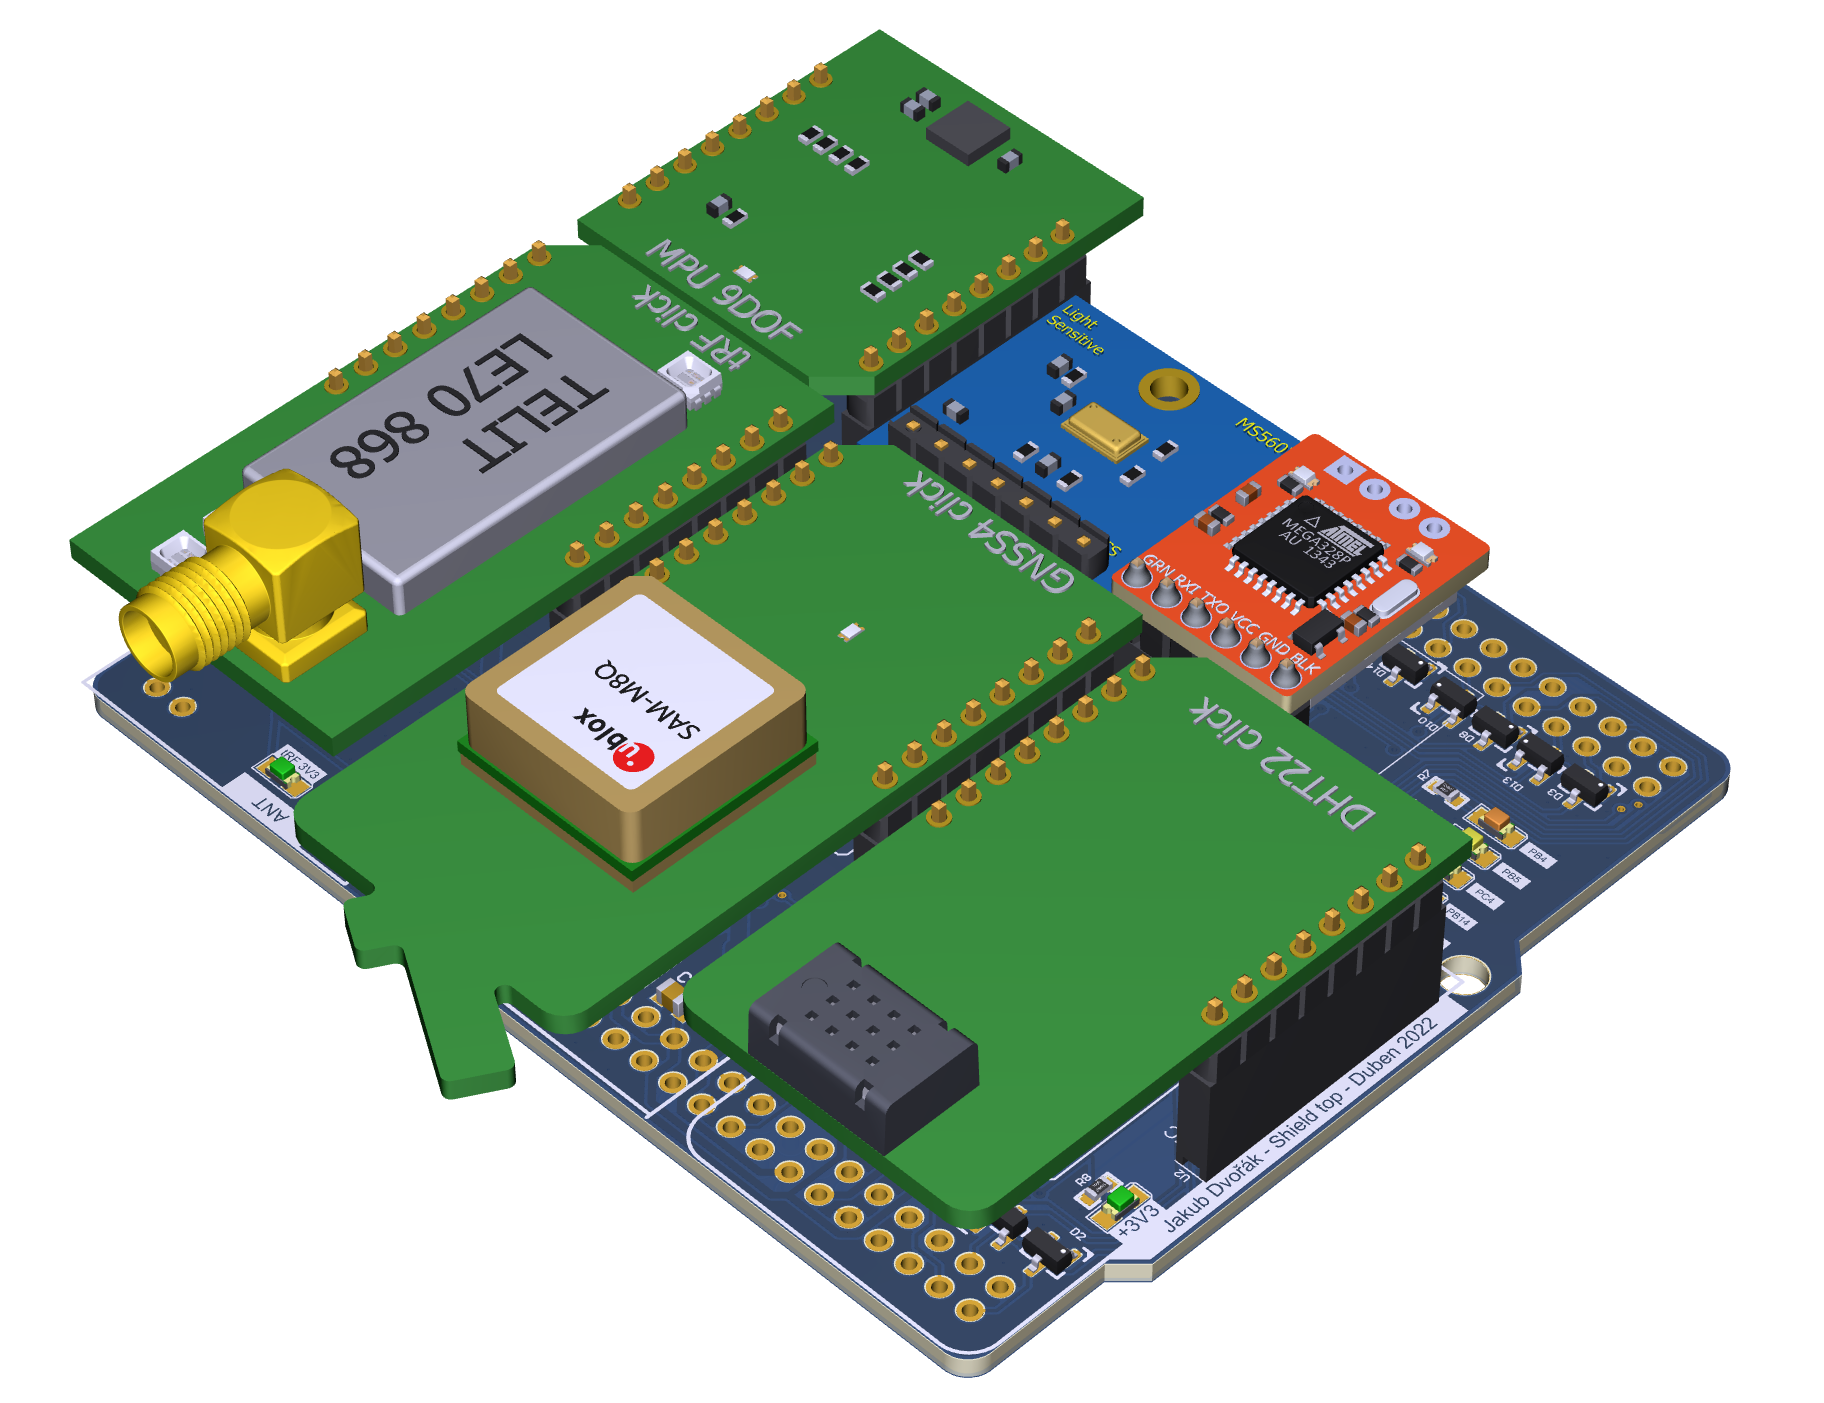
\includegraphics[height=0.7\linewidth]{Figures/shield_top.png} 
				\caption{Vrchní redukční deska}
				\label{fig:shield:top}
			\end{subfigure}%
			\begin{subfigure}{.3\textwidth}
				\centering
				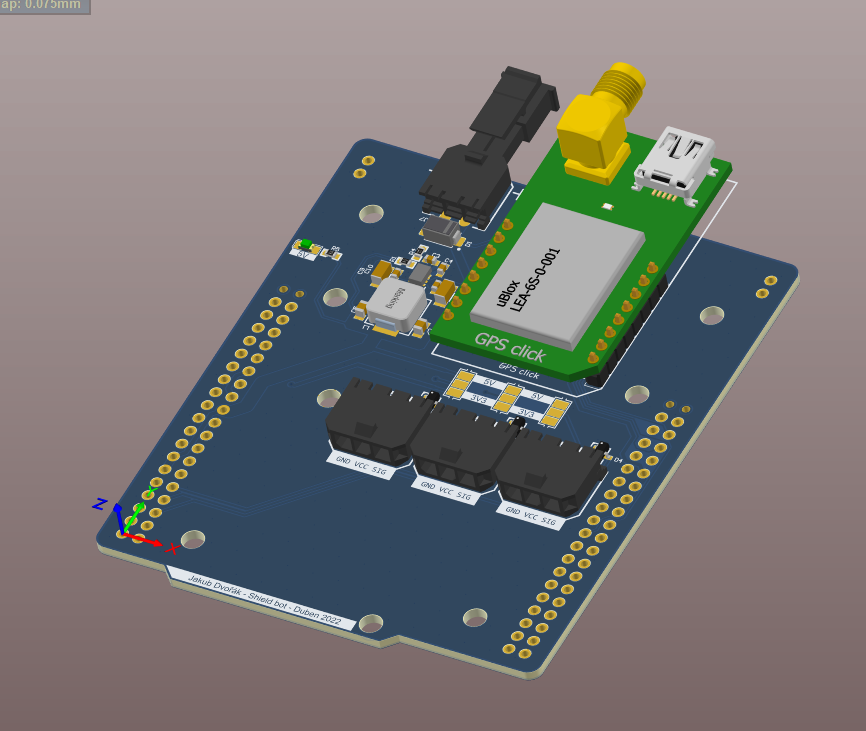
\includegraphics[height=0.7\linewidth]{Figures/shield_bot.png}
				\caption{Spodní redukční deska}
				\label{fig:shield:bot}
			\end{subfigure}
			\begin{subfigure}{.3\textwidth}
				\centering
				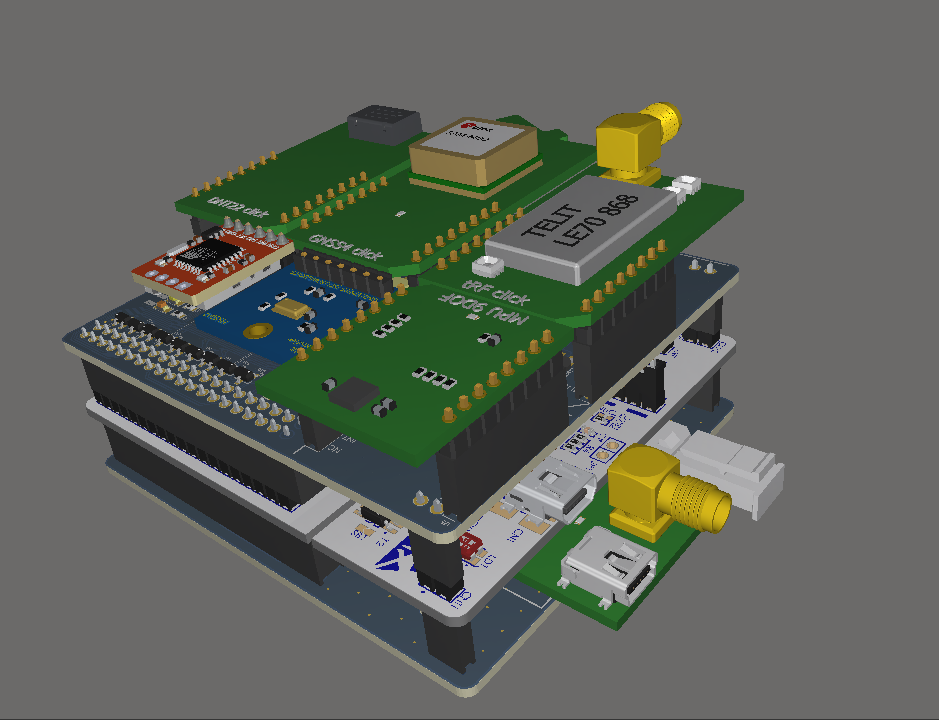
\includegraphics[height=0.7\linewidth]{Figures/shield_assembly.png}
				\caption{Sestava DPS}
				\label{fig:shield:assembly}
			\end{subfigure}
			\caption{Redukční desky pro moduly}
			\label{fig:shields:DPS}
		\end{figure}



		
		\subsection{Napájení}
		Jako zdroj energie po dobu letu byly vybrány tužkové baterie \textit{Energizer ultimate lithium}. Dle technického listu \cite{dsh:AA} jsou schopny operovat až do teploty -40~°C při poklesu kapacity z xxx na xxx mAh. S ohledem na teploty panující ve stratopauze, které klesají až k -60~°C, byl počet zvýšen na 10 ks, nechávající kapacitní rezervu. 

			\subsubsection{Zdroje}
			Vstupní napětí se v závislosti na teplotě a momentálním odběru pohybuje od 18~V do 10~V. Pro zvýšení účinnosti byl jako hlavní regulátor využit spínaný zdroj. S ohledem na dostupnost součástek a ověřenost funkčnosti byl vybrán spínaný zdroj \textit{LMR33630} od firmy \textit{Texas Instruments}. Účinnost tohoto zdroje se pohybuje pro přítomná napájecí napětí od viz graf na obr.~\ref{graf:lmr}.
			\begin{figure}[hbtp]
				\centering
				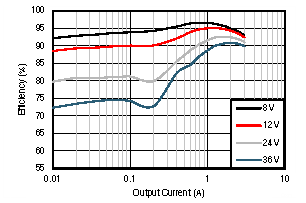
\includegraphics[width=.6\textwidth]{Graphs/lmr33630eff.pdf}
				\caption{Závislost účinnosti na výstupním napětí pro daná vstupní napětí a výstupní napětí $V_\mt{out}= 5\mt{ V}$, převzato z \cite{dsh_lmr}}
				\label{graf:lmr}
			\end{figure}

			Další výhodou spínaného zdroje je minimální PSRR - \textit{Power Source Rejection Ratio}. Výstupní napětí zůstává konstantní bez ohledu na změnu napětí na vstupu, dokud není překročeno minimální napájecí napětí - v našem případě rovno výstupnímu napětí. Limitace čipu je poté 3{,}8~V \cite{dsh_lmr}.
			
			Nevýhodou spínaných zdrojů je zanášení šumu do obvodu. Tento problém se vyřeší využitím lineárního regulátoru. Šum generovaný spínacím regulátorem by mohl způsobit nesprávné fungování mikroprocesoru a snižovat kvalitu příjmu GPS modulu. V tomto případě byla napájecí topologie následující. Napětí baterií bylo na spodní redukční desce spínacím regulátorem sníženo na 5~V. Toto napětí bylo následně skrze nevyužité piny vývojového kitu Nucleo přivedeno na horní redukční desku, kde bylo lineárním regulátorem sníženo na 3{,}3~V. Celkem jsou na desce tři větve s tímto napětím. Mikrokontrolér a senzory mají vlastní větev. Další lineární regulátor napájí pouze GPS modul a třetí lineární regulátor je určen pro radiový vysílač. Díky tomu nebude docházet k poklesu napětí napájení ve zbytku přístroje při vysílání dat. 

			\begin{figure}
				\centering
				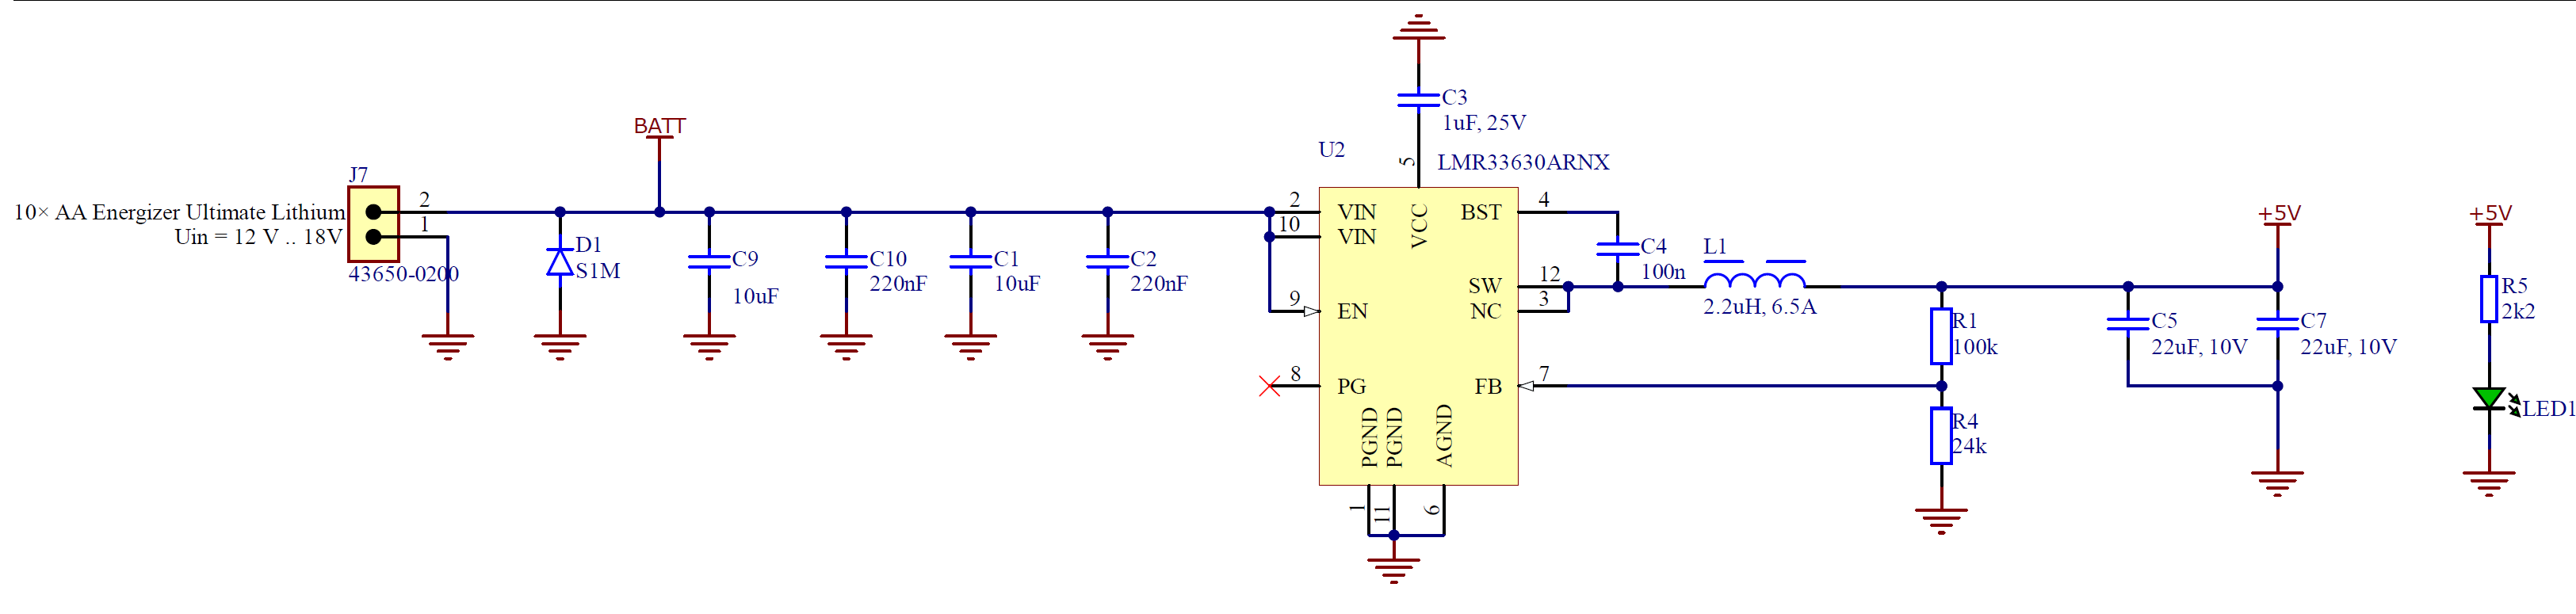
\includegraphics[width = \textwidth]{Figures/psu_bot.png}
				\caption{Schéma spínaného zdroje umístěného na spodní redukční desce}
				\label{fig:psu:bot}
			\end{figure}
			\begin{figure}
				\centering
				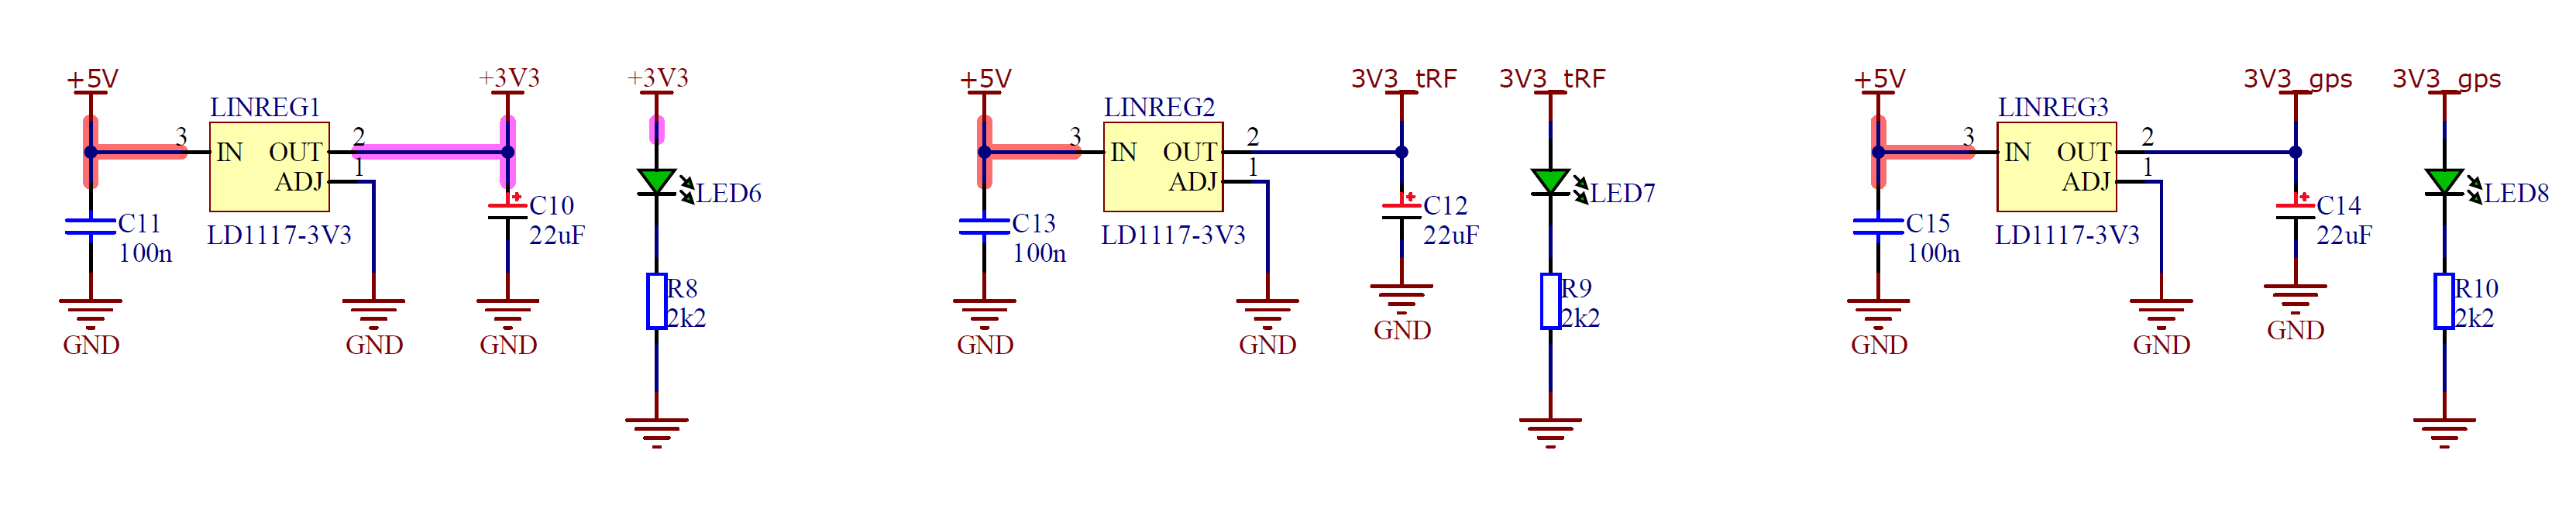
\includegraphics[width = \textwidth]{Figures/psu_top.png}
				\caption{Schéma lineárních regulátorů umístěných na horní redukční desce}
				\label{fig:psu:top}
			\end{figure}


		\subsection{Ochrana pinů}
		Jelikož většina pinů využívaných ke komunikaci byla snadno dostupná na dotyk při manipulaci, bylo potřeba je ošetřit vůči elektrostatickému výboji (ESD), který by měl za následek zničení čipu. Příklad ošetření GPIO pinů pomocí TVS diody BAV99 je na obr. \ref{fig:osetreni:vstupu}.
		
		\begin{figure}
			\centering
			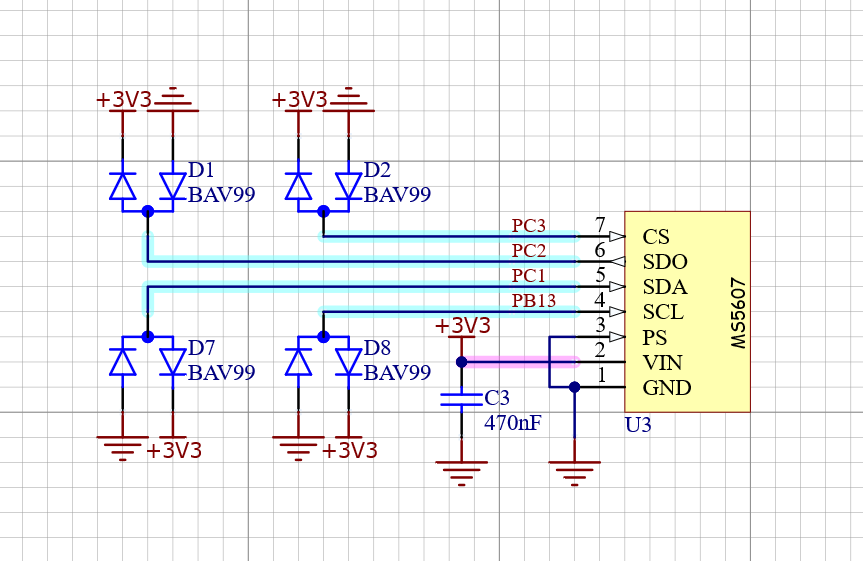
\includegraphics[width = .7\textwidth]{Figures/osetreni_vstupu.png}
			\caption{Příklad ošetření vstupů TVS diodami}
			\label{fig:osetreni:vstupu}
		\end{figure}




	\section{Mechanická zástavba}
	%Součástí práce je i mechanická zástavba kryt pro elektroniku. 
	Pro přehlednost a optimální model krytu bylo potřeba vymodelovat i jednotlivé moduly. Kolem přesného 3D modelu elektroniky mohl být poté vymodelován kryt bez nutnosti čekat na výrobu DPS.
	\begin{figure}[hbtp]
		\centering
		\begin{subfigure}{.5\textwidth}
			\centering
			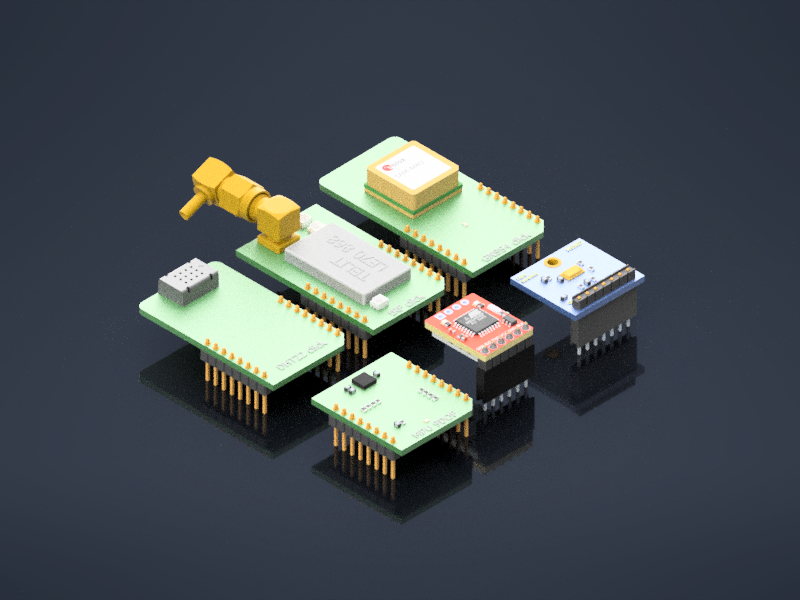
\includegraphics[height=.7\linewidth]{Figures/modules_assembly.png} 
			\caption{Vymodelované moduly}
			\label{fig:modules:assembly}
		\end{subfigure}%
		\begin{subfigure}{.5\textwidth}
			\centering
			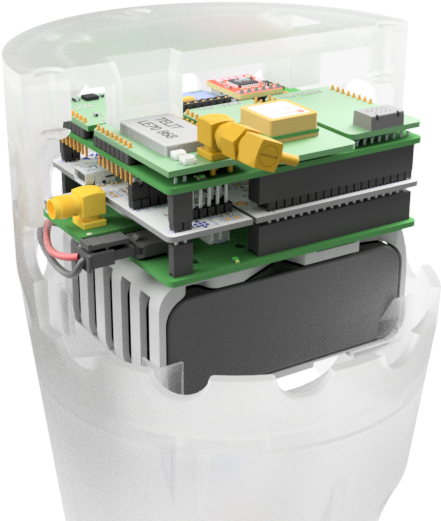
\includegraphics[height=.7\linewidth]{Figures/ALL_rez_white.png}
			\caption{Řez vrchní částí krytu sondy}
			\label{fig:all:rez}
		\end{subfigure}
		\label{fig:shields}
	\end{figure}

	
	Díky jednotlivým modelům bylo možné vytvořit kompletní model elektronické části, kolem kterého byl poté vymodelován kryt (obr. \ref{fig:all:rez}). Kryt byl modelován s ohledem na anténu umístěnou ve spodní části. Stěny kolem antény jsou ztenčené, aby co nejméně ovlivnily ladění antény na 868~MHz. Malá mechanická odolnost stěn je kompenzována čtyřmi výztužemi vedoucí po obvodu stěny.

	Pro splnění hmotnostního limitu byl model krytu postupně odlehčován. Při ubírání materiálu bylo nutné brát v potaz, že hlavní původ velké hmotnosti není při 3D tisku objem tělesa, ale jeho stěny. Při tvorbě otvorů v modelu se tedy neušetřila hmotnost odpovídající objemu válce odebraného ze stěny, ale pouze dvěma jeho podstavám. Naopak materiál byl potřeba na plášť odebraného válce.

	%TODO: názorný jednoduchý model s dírou a bez, iterace 

	Připojení sondy ČHMÚ bylo provedeno pomocí gumového pásu, do kterého se zastrčila skoba odvíječe. To je zařízení, které zajistí postupné odmotání 50m lanka. 50~m je vzdálenost daná výrobcem, která musí být od balónu a dalších součástí sondy, aby byla zajištěna validní měření.

	TODO: obrázek připojení sondy

	V případě, že by došlo k delaminaci 3D tisku, byla jak elektronika, tak sonda ČHMÚ přivázána pojistným provázkem uchyceným k hlavnímu závěsu spolu s padákem a balónem. Díky tomu by sonda stále zůstala pohromadě i když by došlo k rozbití/rozlomení krytu.

	%model DPS, model sondy, iterace, odlehčování, připojení sondy čhmú, bezpečnostní závěsy










	\section{Firmware sondy}
	
		\subsection{Obsluha senzorů}
		Pro vyčítání dat ze senzorů bylo potřeba napsání driveru. Ten má za úkol jak vyčtení dat ze senzoru, tak jeho samotnou inicializaci a nastavení. 

		Výčet dat ze senzoru AM2320 probíhá příkazem
		\lstinputlisting[language=C]{Code/am2320_write.txt}

		Senzor následně vyšle data obsahující informace o vlhkosti a teplotě. Jejich příjem zajišťuje funkce
		\lstinputlisting[language=C]{Code/am2320_read.txt}

		Způsob přepočtu získaných dat na hodnoty teploty a tlaku je popsán v dokumentaci senzoru. Kód pro přepočet je následující:
		\lstinputlisting[language=C]{Code/am2320_get_values.txt}

		Pro senzor teploty a tlaku MS5607 je způsob výčtu dat obdobný. Nejdříve se pošle žádost o převod hodnoty jdoucí ze senzoru.
		\lstinputlisting[language=C]{Code/ms5607_convert_press.txt}
		Následně se pošle žádost o vyčtení hodnot 24bit analogově digitálního převodníku pomocí následujícího kódu.
		\lstinputlisting[language=C]{Code/ms5607_get_press.txt}

		Hodnoty změřené tímto způsobem jsou nekompenzované a jsou ovlivněny nelinearitou senzoru. Pro správnou kompenzaci teploty a tlaku je zapotřebí využít vývojový diagram na obr. \ref{fig:ms5607:flowchart}.
		\begin{figure}
			\centering
			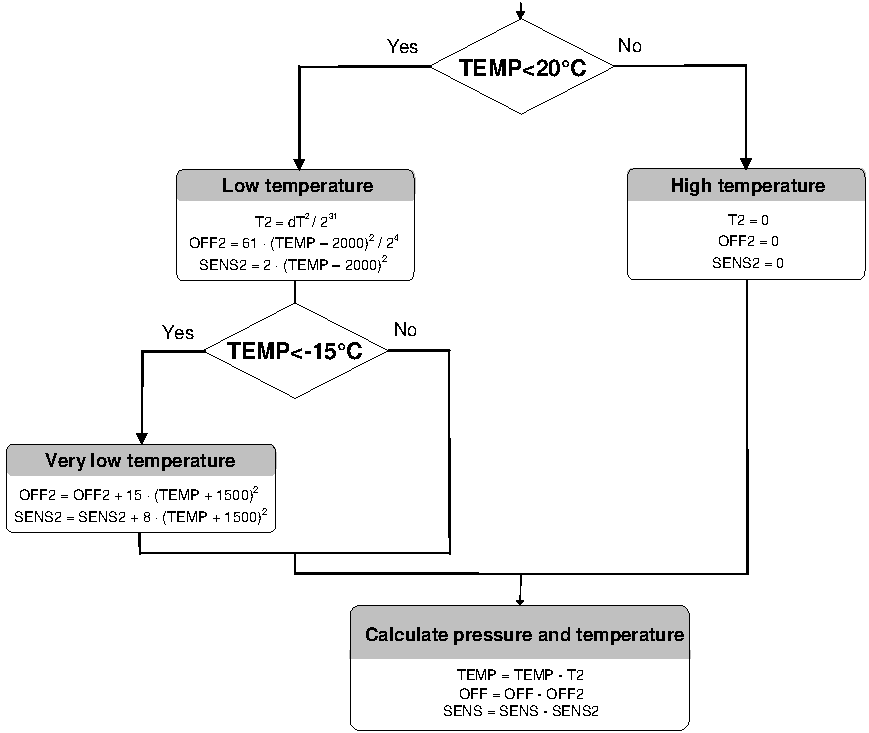
\includegraphics[width=.7\textwidth]{Figures/MS5607_flowchart.pdf}
			\caption{Vývojový diagram pro kompenzaci měřených hodnot senzorem MS5607, převzato z \url{https://www.parallax.com/package/altimeter-module-ms5607-datasheet/}}
			\label{fig:ms5607:flowchart}
		\end{figure}

		Na rozdíl od předešlých senzorů, tento senzor měří hodnoty a ukládá je do příslušných registrů průběžně. Registry senzoru jsou popsány v dokumentu \url{https://invensense.tdk.com/wp-content/uploads/2015/02/RM-MPU-9250A-00-v1.6.pdf}. Slouží k nastavení senzoru samotného, jeho identifikaci a k výčtu naměřených dat. U senzoru je potřeba nastavit vzorkovací frekvenci, rozsahy měřených hodnot a zdroj hodin. Pro následný přístup k datům na dané adrese se využije následujícího příkazu.
		\lstinputlisting[language=C]{Code/MPU_read_CMD.c}
		Senzor následně vyšle hodnoty daného registru a jejich příjem proběhne pomocí funkce níže. Hodnoty ReadAddr a READWRITE\_CMD jsou definovány v \url{https://invensense.tdk.com/wp-content/uploads/2015/02/RM-MPU-9250A-00-v1.6.pdf}.
		\lstinputlisting[language=C]{Code/MPU_read.c}
		


		\subsection{Rozebírání GPS dat}
		Data jsou GPS přijímačem posílána každou sekundu přes sériovou linku ve formátu NMEA zpráv (\url{https://www.sparkfun.com/datasheets/GPS/NMEA%20Reference%20Manual-Rev2.1-Dec07.pdf}). Jedná se o standardizovaný formát GPS dat specifikovaný organizací NMEA (\textbf{N}ational \textbf{M}arine \textbf{E}lectronics \textbf{A}ssociation). Příklad NMEA zpráv je zanesen níže.
		\begin{table}[h!]
			\centering
			\begin{tabular}{l}
				\$GPRMC,132456.00,A,5005.77089,N,01421.46534,E,1.157,,290122,,,A*78\\
				\$GPVTG,,T,,M,1.157,N,2.144,K,A*22\\
				\$GPGGA,132456.00,5005.77089,N,01421.46534,E,1,05,1.79,294.0,M,44.4,M,,*5D\\
				\$GPGSA,A,3,17,06,24,02,15,,,,,,,,2.46,1.79,1.70*0B\\
				\$GPGSV,4,1,13,02,11,134,21,06,20,090,23,10,02,270,,11,06,128,19*76\\
				\$GPGSV,4,2,13,12,70,261,,15,10,185,15,17,17,041,13,19,37,054,*7B\\
				\$GPGSV,4,3,13,22,10,325,,24,72,147,23,25,31,257,08,28,08,068,21*7B\\
				\$GPGSV,4,4,13,32,25,313,*4C\\
				\$GPGLL,5005.77089,N,01421.46534,E,132456.00,A,A*69\\
			\end{tabular}
		\end{table}

		Příklad formátu \$GPGLL zprávy je v tabulce . Informace obsažené v této zprávě jsou vysvětleny v tabulce \ref{tab:gpgll}.
		\begin{longtable}[c]{|l|l|l|}
			\caption{Formát \$GPGLL zprávy}
			\label{tab:gpgll}\\
			\hline
			\rowcolor[HTML]{e5ecf6} 
			\multicolumn{1}{|c|}{\cellcolor[HTML]{DEDFF4}Název} &
			\multicolumn{1}{c|}{\cellcolor[HTML]{DEDFF4}Příklad} &
			\multicolumn{1}{c|}{\cellcolor[HTML]{DEDFF4}Popis} \\ \hline
			\endhead
			%
			Identifikátor zprávy & \$GPGLL     & GLL hlavička \\ \hline
			Zem. Šířka           & 5005.77089  & ddmm.mmmm    \\ \hline
			N/S (Sever/Jih)      & N           &              \\ \hline
			Zem. Délka           & 01421.46534 & dddmm.mmmm   \\ \hline
			E/W (Východ/Západ)   & E           &              \\ \hline
			UTC Čas              & 132456.00   & hhmmss.sss   \\ \hline
			Status &
			A &
			\begin{tabular}[c]{@{}l@{}}A - data jsou validní\\ V  data nejsou   validní\end{tabular} \\ \hline
			Mód &
			A &
			\begin{tabular}[c]{@{}l@{}}A - autonomous\\ D - DGPS\\ E - DR\end{tabular} \\ \hline
			Kontrolní součet             & *69         &              \\ \hline
			<CR> <LF>            &             & Konec zprávy \\ \hline
		\end{longtable}

		Délka zprávy odeslané GPS přijímačem se liší podle dostupných údajů. Pokud GPS nezná svou polohu, pole pro zeměpisnou šířku a délku jsou prázdná. Proto nemůžeme očekávat zprávy fixní velikosti. Způsob, kterým se ve firmwaru sondy NMEA zpráva přijímá je znározněn v ukázce kódu \ref{code:ReceiveToIdle}.
		\lstinputlisting[language=C, caption={Funkce pro příjem dat z GSP}, label={code:ReceiveToIdle}]{Code/HAL_UARTEx_ReceiveToIdle_IT.c}

		Tato funkce přijímá data až do doby, kdy nenastane klidový stav - GPS přestane vysílat data. V ten moment se vyvolá callback funkce.
		\lstinputlisting[language=C,caption={Callback funkce vyvolaná interruptem}, label={lst:main:callback}]{Code/callback.c}
		V této funkci se do globální proměnné \lstinline[language=C] |uint16_t DataRecieved | uloží velikost přijatých dat. Pokud je v hlavní smyčce programu splněna podmínka, že \lstinline[language=C] |  DataRecieved > 0 |, program začne rozebírání přijatých dat funkcí \ref{lst:main:parse}. Pro rozdělení přijatých dat na jednotlivé NMEA zprávy se využívá znaků <CR> <LF>, které se nacházejí na konci každého řádku. 
		
		Součástí vyslaných dat jsou i \$GPGSV zprávy obsahující informace o viditelných satelitech. Zpráv tohoto typu je vysílá několik po sobě a počet vyslaných zpráv je zanesen v prvním poli této zprávy. Pro správně rozdělení přijatých dat je informace o počtu \$GPGSV zpráv nutná, jelikož ovlivňuje pořadí dalšách zpráv.

		Funkce \lstinline[language=C] |mainParse| v ukázce \ref{lst:main:parse} rozdělí a uloží data do bufferu \lstinline |uint8_t GPSparse[15][200] = {}|   tvořeného 2D polem a zjistí počet \$GPGSV zpráv.

		\lstinputlisting[language=C++,caption={Hlavní parsovací funkce}, label={lst:main:parse}]{Code/main_parse.c}



		Příklad volání funkce v hlavní smyčce programu je znázorněn v ukázce kódu \ref{lst:main:loop}.
		\lstinputlisting[language=C, caption={Volání funkcí v hlavní smyčce programu}, label={lst:main:loop}]{Code/parse_in_main.txt}

		Ve stejné větvi programu, kde se vykonává rozebírání NMEA zpráv, se vyčtou data ze senzorů. Tyto číslené hodnoty se poté převedou do textové podoby a přidají mezi vysílaná data. Převod z číselné hodnoty na textovou, obsahující ASCII znaky, slouží funkce \lstinline |ftoa()|, která převádí číslo typu float a funkce \lstinline[language=C] |itoa()| pro převod čísla typu int. 

		Z rozebraných NMEA zpráv jsou poté vybrána data, která se spolu s naměřenými hodnotami ze senzorů, převedené do textové podoby, sešijí do první zprávy. Tato zpráva se posléze pošle skrze sériovou linku do radiového vysílače. K této zprávě se po odeslání přidají další data a zpráva je poslána do záznamníku, kde se uloží na SD kartu v lidsky čitelném formátu. Příklady vysílaných zpráv jsou v tabulkách \ref{tab:TX} a \ref{tab:SD}.

		%telit data
		\begin{table}[h]
			\centering
			\resizebox{\textwidth}{!}{%
			\caption{Formát telemetrické zprávy}
			\label{tab:TX}
			\begin{tabular}{|l|ll|ll|l|l|l|l|}
			\hline
			\rowcolor[HTML]{E5ECF6} 
			\multicolumn{1}{|c|}{\cellcolor[HTML]{E5ECF6}UTC čas} &
			\multicolumn{2}{c|}{\cellcolor[HTML]{E5ECF6}Zem. šířka (°)} &
			\multicolumn{2}{c|}{\cellcolor[HTML]{E5ECF6}Zem. Délka (°)} &
			\multicolumn{1}{c|}{\cellcolor[HTML]{E5ECF6}\begin{tabular}[c]{@{}c@{}}Nadmořská výška\\ (m)\end{tabular}} &
			\multicolumn{1}{c|}{\cellcolor[HTML]{E5ECF6}\begin{tabular}[c]{@{}c@{}}Ryhlost\\ (m/s)\end{tabular}} &
			\multicolumn{1}{c|}{\cellcolor[HTML]{E5ECF6}\begin{tabular}[c]{@{}c@{}}Teplota\\ (°C)\end{tabular}} &
			\multicolumn{1}{c|}{\cellcolor[HTML]{E5ECF6}\begin{tabular}[c]{@{}c@{}}Tlak\\ (Pa)\end{tabular}} \\ \hline
			114231.00 &
			\multicolumn{1}{l|}{5001.76165} &
			N &
			\multicolumn{1}{l|}{01430.16855} &
			E &
			9510.0 &
			23.428 &
			-039.65 &
			0028254 \\ \hline
			\multicolumn{9}{c}{}\\
			\multicolumn{9}{c}{Přijatá zpráva: \lstinline |114231.00;5001.76165;N;01430.16855;E;9510.0;23.428;-039.65;0028254|}
			\end{tabular}%
			}
			\end{table}

		%SD data
		\begin{table}[]
			\caption{Formát dat ukládaných na SD kartu}
			\label{tab:SD}
			\centering
			\resizebox{\textwidth}{!}{%
			\begin{tabular}{|l|ll|ll|l|l|l|l|l|l|l}
			\hline
			\rowcolor[HTML]{E5ECF6} 
			\multicolumn{1}{|c|}{\cellcolor[HTML]{E5ECF6}UTC čas} &
			\multicolumn{2}{c|}{\cellcolor[HTML]{E5ECF6}Zem. šířka (°)} &
			\multicolumn{2}{c|}{\cellcolor[HTML]{E5ECF6}Zem. Délka (°)} &
			\multicolumn{1}{c|}{\cellcolor[HTML]{E5ECF6}\begin{tabular}[c]{@{}c@{}}Nadmořská výška\\ (m)\end{tabular}} &
			\multicolumn{1}{c|}{\cellcolor[HTML]{E5ECF6}\begin{tabular}[c]{@{}c@{}}Ryhlost\\ (m/s)\end{tabular}} &
			\multicolumn{1}{c|}{\cellcolor[HTML]{E5ECF6}\begin{tabular}[c]{@{}c@{}}Teplota\\ (°C)\end{tabular}} &
			\multicolumn{1}{c|}{\cellcolor[HTML]{E5ECF6}\begin{tabular}[c]{@{}c@{}}Tlak\\ (Pa)\end{tabular}} &
			\multicolumn{1}{c|}{\cellcolor[HTML]{E5ECF6}\begin{tabular}[c]{@{}c@{}}Teplota 2\\ (°C)\end{tabular}} &
			\multicolumn{1}{c|}{\cellcolor[HTML]{E5ECF6}\begin{tabular}[c]{@{}c@{}}Relativní vlhkost\\ (\%)\end{tabular}} &
			\multicolumn{1}{c}{\cellcolor[HTML]{E5ECF6}\begin{tabular}[c]{@{}c@{}}Typ GPS\\ fixu\end{tabular}} \\ \hline
			114231.00 &
			\multicolumn{1}{l|}{5001.76165} &
			N &
			\multicolumn{1}{l|}{01430.16855} &
			E &
			9510.0 &
			23.428 &
			-039.65 &
			0028254 &
			-40.5 &
			003.2 &
			2 \\ \hline
			\end{tabular}
			}
			\begin{tabular}{c}
				~
			\end{tabular}
			\resizebox{\textwidth}{!}{%
			\begin{tabular}{l|l|l|l|l|lll|lll|lll|}
				\hline
				\rowcolor[HTML]{E5ECF6} 
				\multicolumn{1}{c|}{\cellcolor[HTML]{E5ECF6}\begin{tabular}[c]{@{}c@{}}Počet viditelných\\ satelitů\end{tabular}} &
				\multicolumn{1}{c|}{\cellcolor[HTML]{E5ECF6}PDOP} &
				\multicolumn{1}{c|}{\cellcolor[HTML]{E5ECF6}HDOP} &
				\multicolumn{1}{c|}{\cellcolor[HTML]{E5ECF6}VDOP} &
				\multicolumn{1}{c|}{\cellcolor[HTML]{E5ECF6}\begin{tabular}[c]{@{}c@{}}Nejmenší změřené\\ zrychlení v ose Z\end{tabular}} &
				\multicolumn{3}{c|}{\cellcolor[HTML]{E5ECF6}Velikost zrychlení} &
				\multicolumn{3}{c|}{\cellcolor[HTML]{E5ECF6}Velikost úhlové rychlosti} &
				\multicolumn{3}{c|}{\cellcolor[HTML]{E5ECF6}\begin{tabular}[c]{@{}c@{}}Velikost intenzity\\ mag. pole\end{tabular}} \\ \hline
				12 &
				1.32 &
				0.70 &
				1.12 &
				7062 &
				\multicolumn{1}{l|}{12} &
				\multicolumn{1}{l|}{-232} &
				8452 &
				\multicolumn{1}{l|}{52} &
				\multicolumn{1}{l|}{-117} &
				245 &
				\multicolumn{1}{l|}{-4218} &
				\multicolumn{1}{l|}{3765} &
				-3276 \\ \hline
				\multicolumn{14}{c}{}\\
				%\multicolumn{14}{c}{Přijatá zpráva: 114231.00;5001.76165;N;01430.16855;E;9510.0;23.428;-039.65;0028254;-40.5;003.2;2;12;1.32;0.70;1.12;7062;12;-232;8452;52;-117;245;-4218;3765;-3276;}
			\end{tabular}
			}
		\end{table}
			


		



		\subsection{Zjištění náklonu sondy}
		Aby bylo možné zjisti, jaká část směrové charakteristiky antény byla využita pro přenos dat, bylo nutné zjisti výchylku sondy od svislé osy. Zjištění výchylky sondy lze realizovat metodami jendoduššími a méně přesnějšími, nebo přesnými, sofistikovanými metodami. 

		Díky přítomnosti modulu 9DOF od firmy \textit{Microelektronika} lze pro měření náklonu využít data z akcelerometru, gyroskopu a magnetometru. Ve statickém případě lze pro výchylku využít pouze akcelerometr. Velikost zrychlení v ose $z$ sondy se bude měnit spolu s vychylováním sondy od svislé polohy. Pro výchylku $\varphi$ platí ve statickém stavu
		\begin{align}
			\varphi = \text{cos}^{-1}\left(\frac{a_z}{g}\right).
		\end{align}
		Pokud se bude sonda kývat kolem pevného bodu, bude na ni působit i odstředivé zrychlení, které se bude přičítat k $a_z$. V tomto případě by šlo zjistit velikost odstředivého zrychlení díky gyroskopu, který měří úhlovou rychlost. Pro odstředivé zrychlení $a_\text{o}$ platí
		\begin{align}
			a_\text{o} = \omega^2 l,
		\end{align}
		kde $\omega$ je úhlová rychlost daná jako $\frac{\diff \varphi}{\diff t}$ a $l$ je délka závěsu sondy. V tomto případě ale nelze stanovit délku závěsu, jelikož balón, za který je sonda přichycena, není pevný bod.

		Jak již bylo řečeno, zjištění výchylky $\varphi$ je možné pouze při statisckém stavu. K němu dochází, kdy se sonda dostane do maximální výchylky a poté se úhel začně opět snižovat. Pokud správně určíme moment, kdy k tomuto stavu došlo, můžeme správně určit maximální výchylku za danou periodu. 

		\begin{figure}[hbtp]
			\centering
			\begin{subfigure}{.49\textwidth}
				\centering
				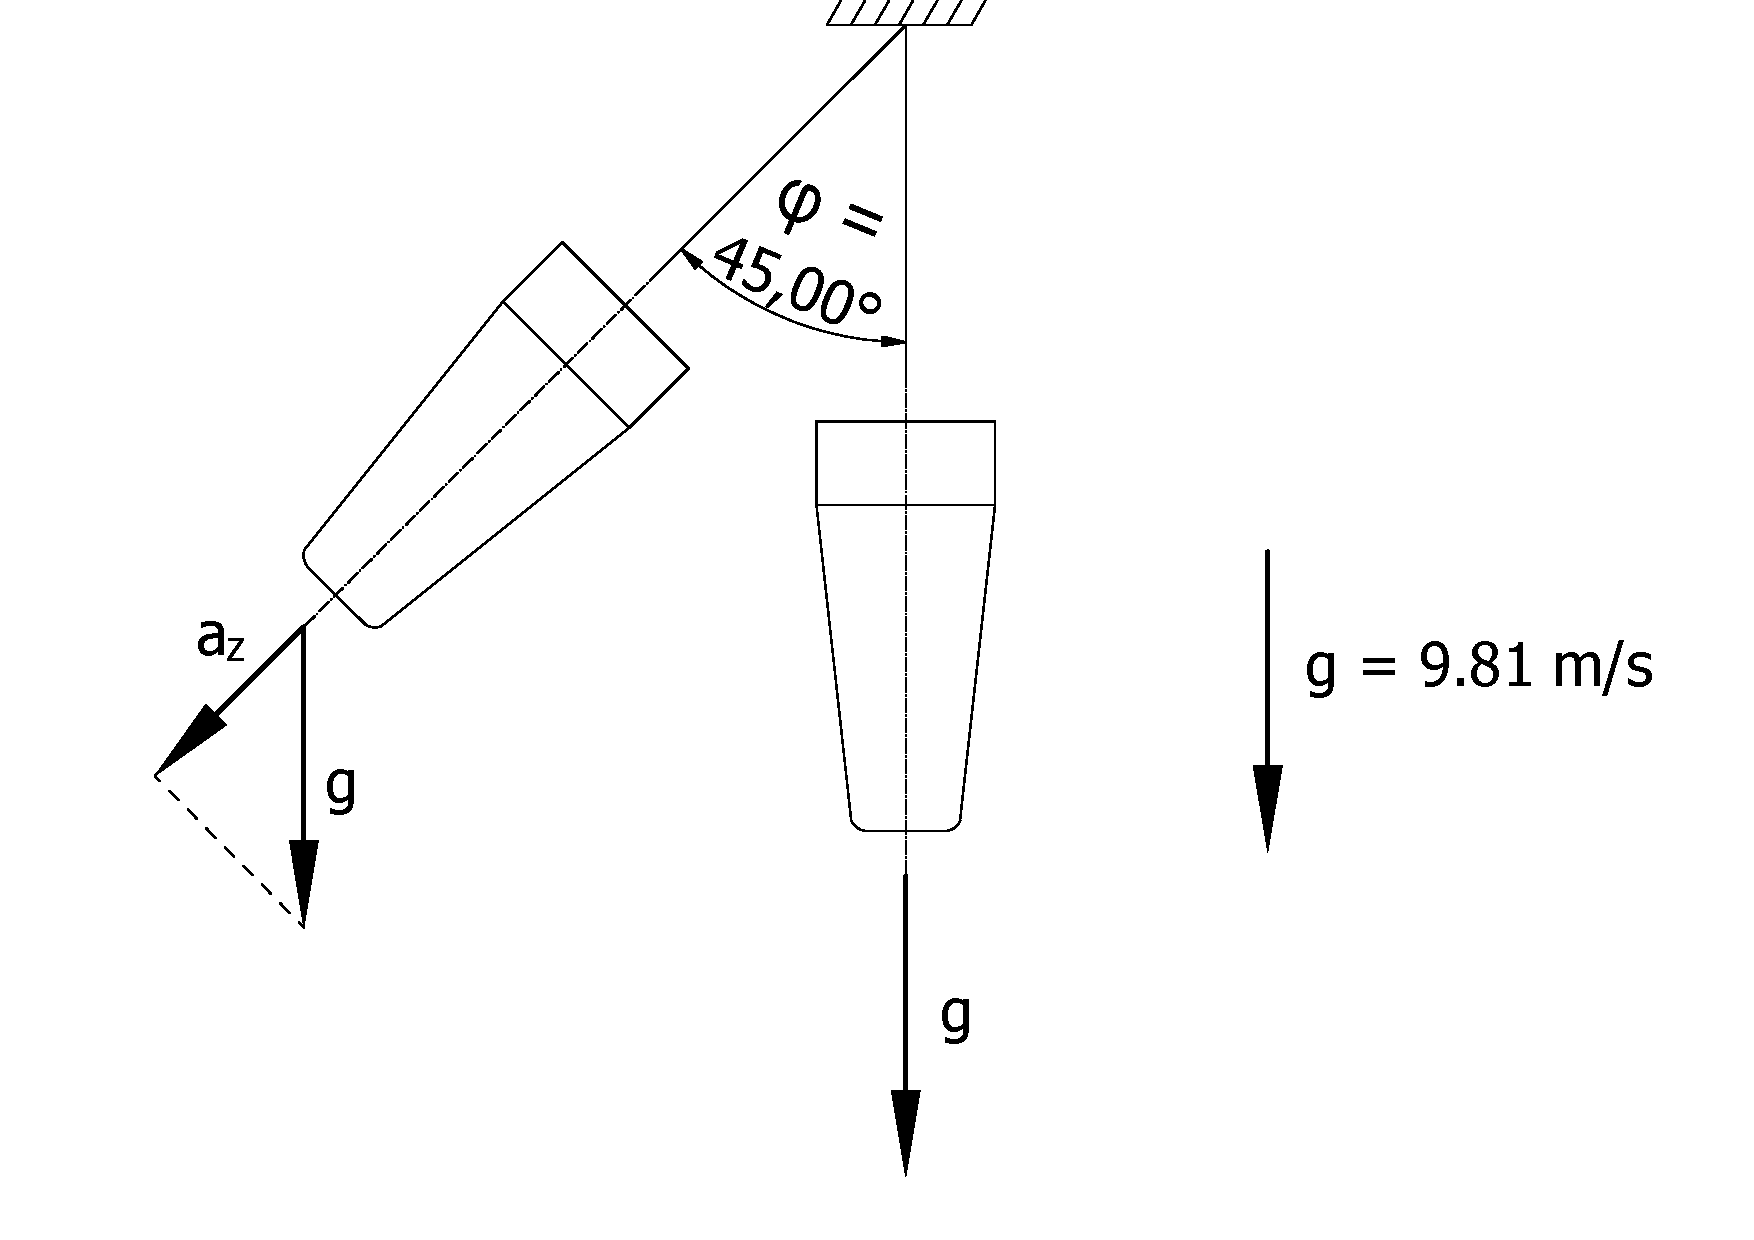
\includegraphics[width=\textwidth]{Figures/sonda_naklon_acc.pdf}
				\caption{Změna zrychlení působící ve směru $z$ při statickém vychýlení}
				\label{fig:sonda:naklon}
			\end{subfigure}%
			\begin{subfigure}{.49\textwidth}
				\centering
				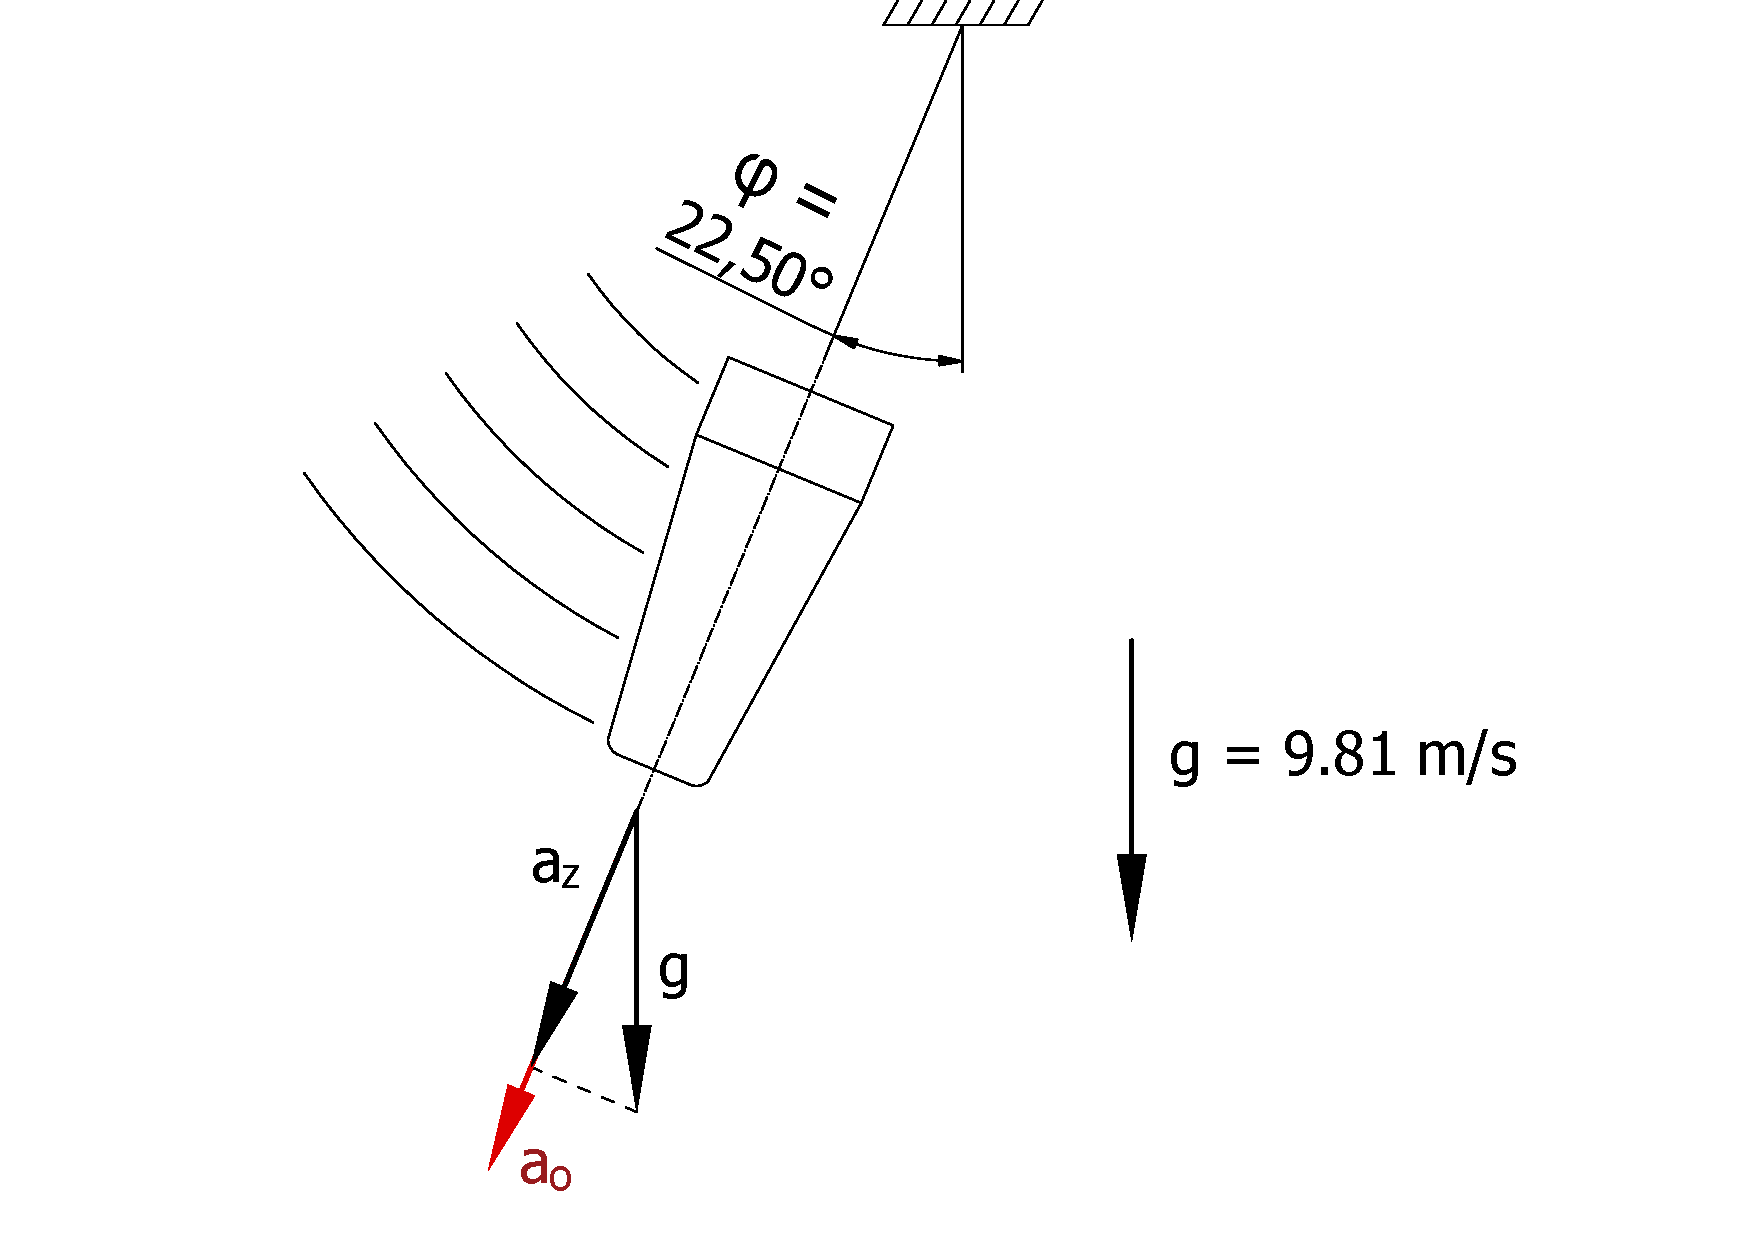
\includegraphics[width=\textwidth]{Figures/sonda_naklon_acc_odst.pdf}
				\caption{Změna zrychlení působící ve směru $z$ při pohybu sondy}
				\label{fig:sonda:naklon:odst}
			\end{subfigure}
			\caption{Zrychlení působící na sondu}
			\label{fig:sonda:naklon:main}
		\end{figure}

		Jak bylo dřívě zmíněno, měření dat probíhá jednou za sekundu a je iniciováno příjmem GPS dat. Mimo tohoto měření jsou s větší frekvencí měřena data o zrychlení sondy a do bufferu je ukládána nejnižší hodnota zrychlení ve směru osy $z$ viz ukázka kódu \ref{lst:sonde:acc}. Funkce \lstinline[language=C]|filter(int *out, int *in, int *b)| je dolní propust prního řádu. Po uměhnutí sekundové periody se minimální hodnota vyčte z bufferu, uloží spolu s dalšími daty na SD kartu a buffer se vynuluje.
			\lstinputlisting[language=C, float=h, caption={Zjištění minimálního zrychlení}, label={lst:sonde:acc}]{Code/sonde_min_acc.c}


		Další řešení, které se nabízelo, bylo zjištění náklonu za pomoci vektoru magnetické indukce. Pro rozsahy vzdáleností, ve kterých se sonda pohybuje, můžeme uvažovat směr vektoru magnetické indukce za konstantní a tedy podle něj určit náklon sondy viz. obr. \ref{fig:sonda:mag}. Na začátku měření je potřeba změřit úhel, kterým vektor magnetické indukce směřuje. Následně pro náklon sondy platí
		\begin{align}
			\varphi = \varphi_\text{meas} - \varphi_\text{ref}.
		\end{align}

		\begin{figure}[hbtp]
			\centering
			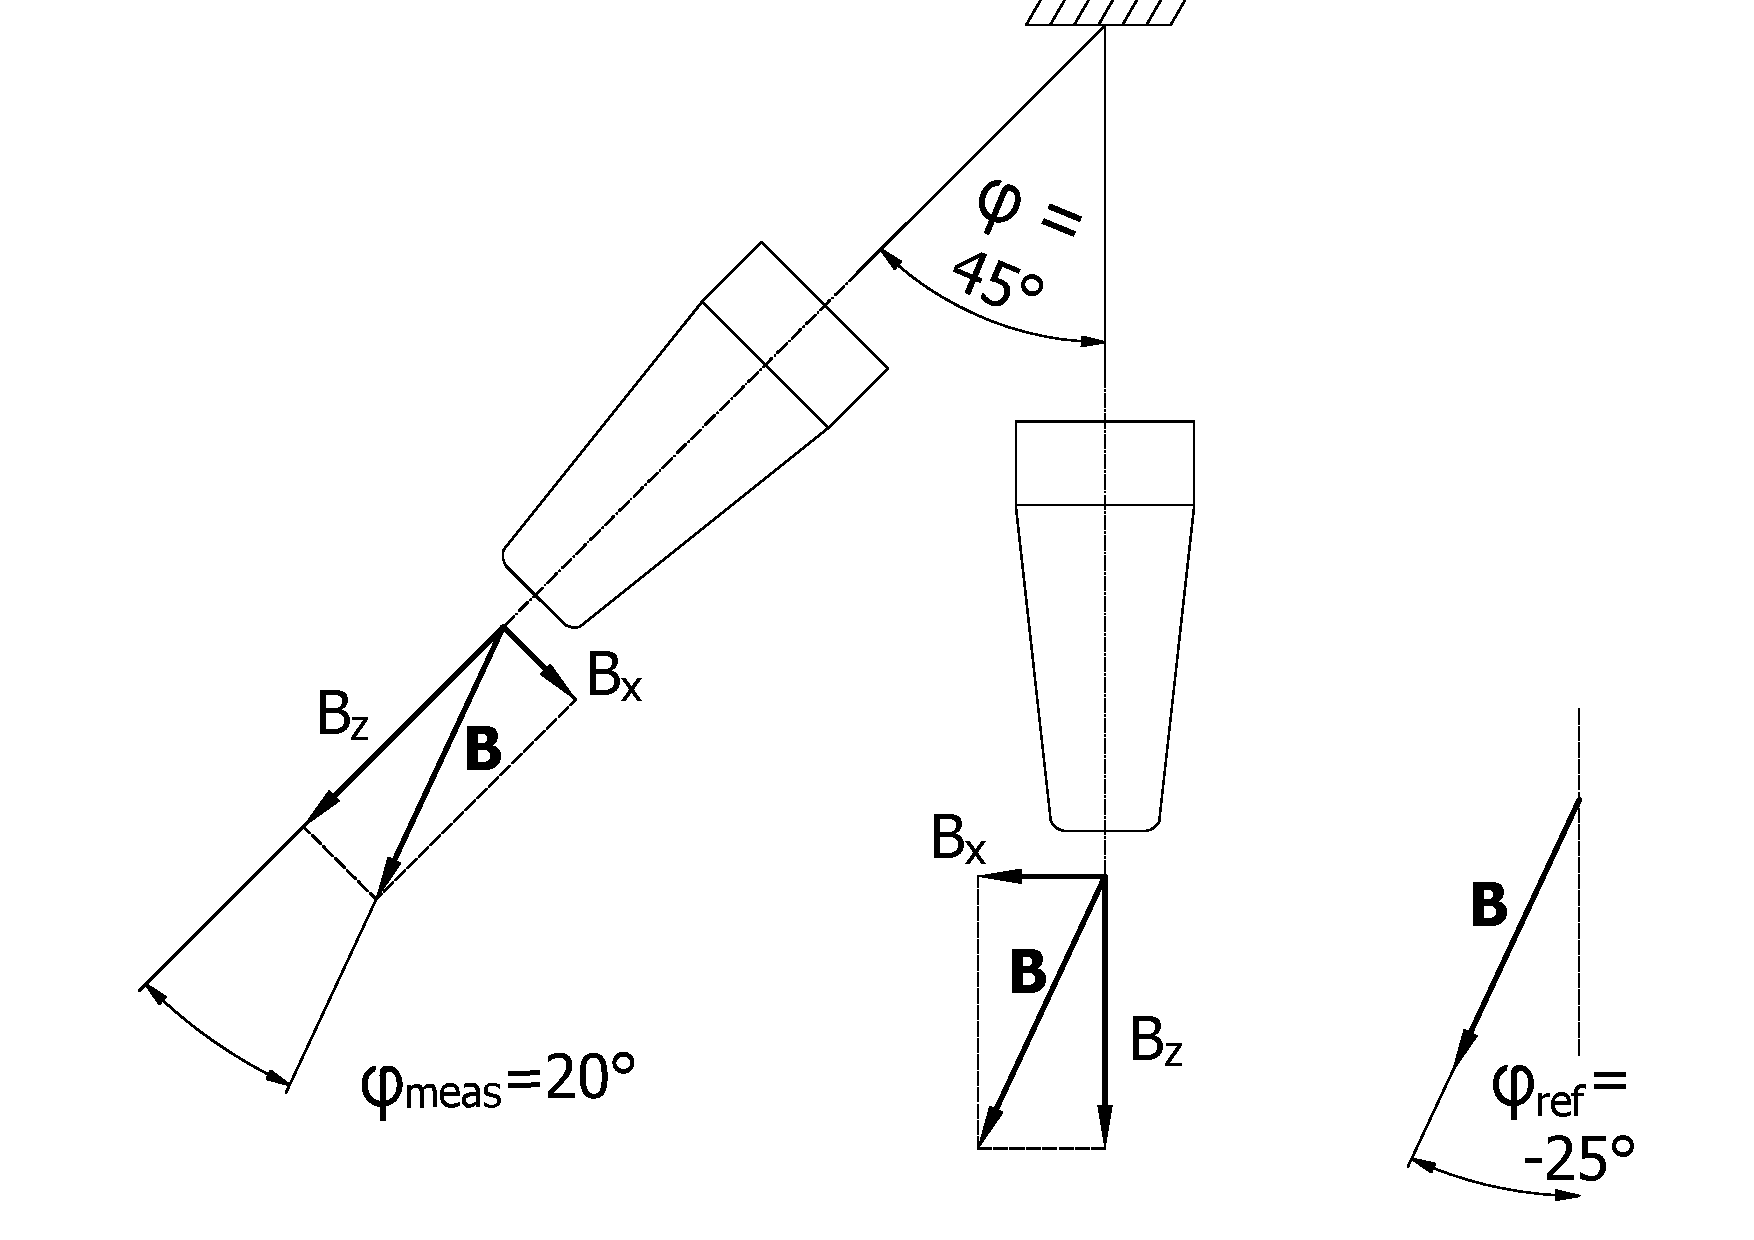
\includegraphics[width=.5\textwidth]{Figures/sonda_naklon_mag.pdf}
			\caption{Měření náklonu sondy pomocí vektoru magnetické indukce}
			\label{fig:sonda:mag}
		\end{figure}

		Tento způsob výpočtu náklonu sondy bohužel funguje pouze ve 2D. Pokud se přesuneme do 3D prostoru, narazíme na následující problém. Při rotaci kolem vektoru magnetické indukce se měřené hodnoty se nebudou měnit, jak je znázorněno na obr.~\ref{fig:sonda:mag:rot}. Tento způsob by šlo použít poze v případě, že by vektor magnetické indukce směřoval svisle k zemi. Při obecné orientaci bohužel tato metoda využít nejde.

		\begin{figure}[hbtp]
			\centering
			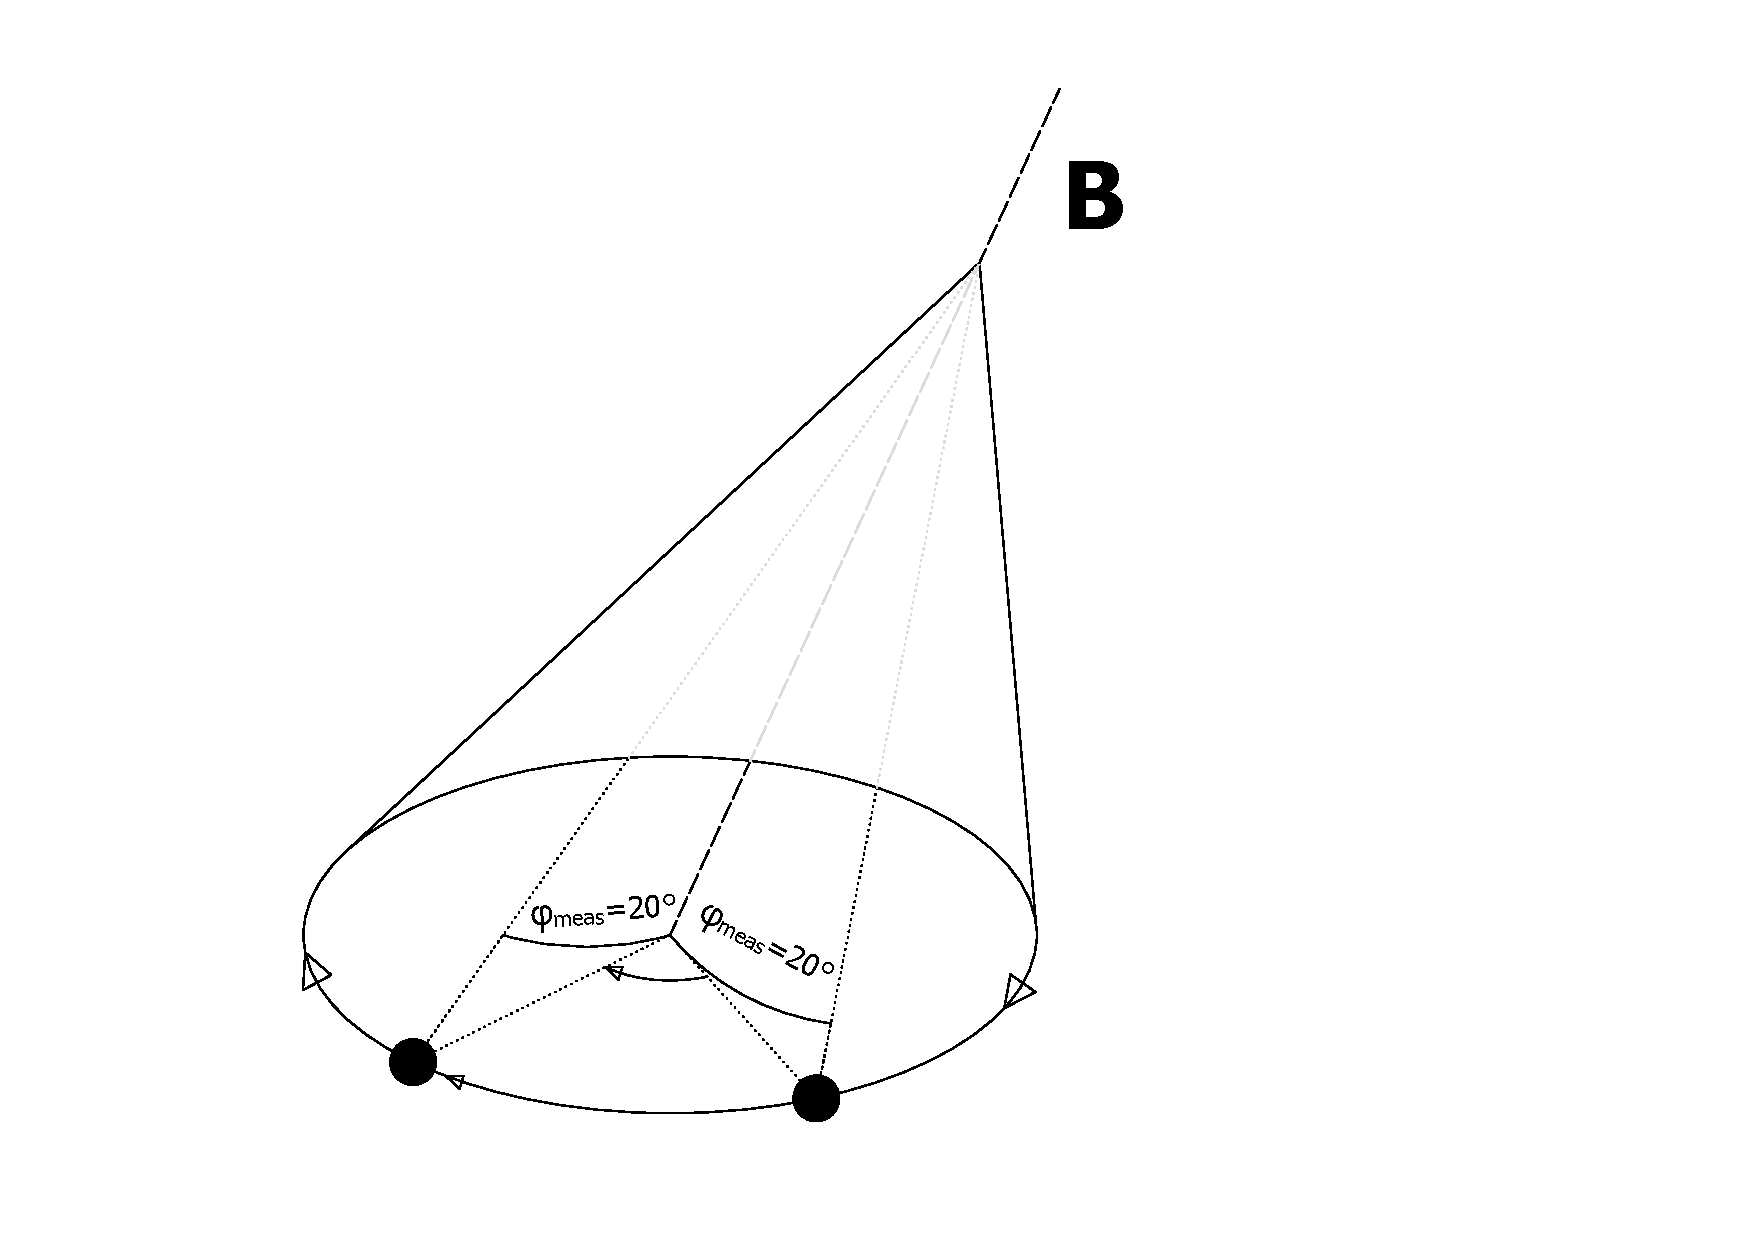
\includegraphics[width=.5\textwidth]{Figures/sonda_naklon_mag_osova_rotace.pdf}
			\caption{Rotace sondy kolem osy tvořené vektorem magnetické indukce (pohled zespod)}
			\label{fig:sonda:mag:rot}
		\end{figure}

		Pro zjištění náklonu je využita první zmíněna metoda. Jelikož není možné zjistit okamžitou výchylku, ale pouze maximální výchylku za dobu jedné periody GPS přijímače, bylo počítáno se standartním rozkmitem sondy, jehož hodnota je bere jako konstatní po celou dobu letu. 
		


	












	
	\section{Realizace pozemní stanice}
	%výstřizky kódu z driverů, sample GPS dat, vyčítání z teplota/tlak, tlak/vlhkost, gyro/acc/mag, parsovací funkce, změřené minimum accelerace v z-ose, sešití dat, watchdog, reset při erroru

	Jak již bylo zmíněno v kapitole \ref{sec:navrh:pozemni_stanice}, úkolem pozemní stanice je překládat přijímaná data zpět do formátu NMEA GPGGA zprávy, určené pro tracker. Rozdělení příchozí zprávy vyslané sondou probíhá obdobně jako v sondě. Přijatá data jsou znak po znaku iterována a zkoumá se, jestli se nenarazilo na oddělovací znak - v tomto případě středník viz ukázka kódu \ref{lst:ground:parse}. Pro samotný příjem dat nelze jako v sondě využít funkce, která přijímá, dokud nenastane prodleva. Vysílací modul sám posílá data po 30 znacích a i mezi těmito balíky dat je prodleva. Zpráva se tedy musí načítat znak po znaku, jak je ukázáno v kódu \ref{lst:ground:recieve}, a jako konec zprávy brát až znak \lstinline |"\n"|.

	\lstinputlisting[language=C, caption={Příjem dat pozemní stanicí}, label={lst:ground:recieve}]{Code/ground_station_read.c}

	\lstinputlisting[language=C, caption={Rozdělení příchozí zprávy do jednotlivých polí}, label={lst:ground:parse}]{Code/ground_station_parse.c}

	Jelikož některé informace, které \$GPGGA zpráva obsahovala, nebyly přeneseny telemetrií, musely být na zemi doplněny. Pro tracker nicméně nejsou důležité a tudíž mohly být jakékoliv. Jedná se o jednotky, odchýlení od geoidu a HDOP - Horizontal Dillution of Precision (Horizontální zředění přesnosti), viz tabulka \ref{tab:gpgga}. Poslední pole, obsahující kontrolní součet muselo být spočítáno podle údajů posílaných do trackeru. Kontrolní součet je podle (https://nmeachecksum.eqth.net/) logický XOR všech znaků mezi znaky \$ a *. Funkce pro výpočet kontrolního součtu je ukázána v kódu \ref{lst:ground:checksum}.

	\lstinputlisting[language=C, caption={Výpočet kontrolního součtu}, label={lst:ground:checksum}]{Code/ground_station_checksum.c}

	%TODO - ukázat na osciloskopu/log analyzátoru balíky dat

	\begin{longtable}[c]{|l|l|l|l|}
	\caption{Formát GPGGA zprávy}
	\label{tab:gpgga}\\
	\hline
	\rowcolor[HTML]{E5ECF6} 
	\multicolumn{1}{|c|}{\cellcolor[HTML]{E5ECF6}Název} &
  	\multicolumn{1}{c|}{\cellcolor[HTML]{E5ECF6}Příklad} &
  	\multicolumn{1}{c|}{\cellcolor[HTML]{E5ECF6}Jednotky} &
  	\multicolumn{1}{c|}{\cellcolor[HTML]{E5ECF6}Popis} \\ \hline
	\endhead
	%
	Identifikátor zprávy          & \$GPGGA     &         & GGA hlavička                \\ \hline
	UTC Čas                       & 132456     &         & hhmmss.sss                  \\ \hline
	Zem. Šířka                    & 5005.77089 &         & ddmm.mmmm                   \\ \hline
	N/S (Sever/Jih)               & N          &         &                             \\ \hline
	Zem. Délka                    & 1421.46534 &         & dddmm.mmmm                  \\ \hline
	E/W (Východ/Západ)            & W          &         &                             \\ \hline
	Druh určení pozice &
	1 &
	&
	\begin{tabular}[c]{@{}l@{}}0 data nejsou validní\\ 1 data jsou validní\\ 2 diferenciáln í GPS\end{tabular} \\ \hline
	Počet využitých satelitů      & 5          &         &                             \\ \hline
	HDOP                          & 1.79       &         &                             \\ \hline
	Nadmořská výška               & 294        & metry   &                             \\ \hline
	Jednotky                      & M          & metry   &                             \\ \hline
	Odchýlení od geoidu           & 44.4       & metry   & Separace geoidu a elipsoidu \\ \hline
	Jednotky                      & M          & metry   &                             \\ \hline
	Stáří rozdílové korekce       & -          & sekundy &                             \\ \hline
	Diff. Ref. Station ID		  & -          &         &                             \\ \hline
	Kontrolní součet              & *5D        &         &                             \\ \hline
	<CR> <LF>                     &            &         & Konec zprávy                \\ \hline
	\end{longtable}











	\section{Software pro zobrazení telemetrických údajů}
	Příjem dat samotných byl realizován stejným modulem, který je unmístěn v sondě, určený k posílání telemetrických dat. Pro minimalizaci ztrát byla anténa s modulem umístěny na platformě, která byla pomocí magnetů uchycena na střeše automobilu obr. \ref{fig:tack:mech:platform}. K modulu byl připojen převodník ze sériové linky na USB, který byl dostatečně dlouhým USB kabelem připojen k laptopu spolujezdce.

	\begin{figure}
		\centering
		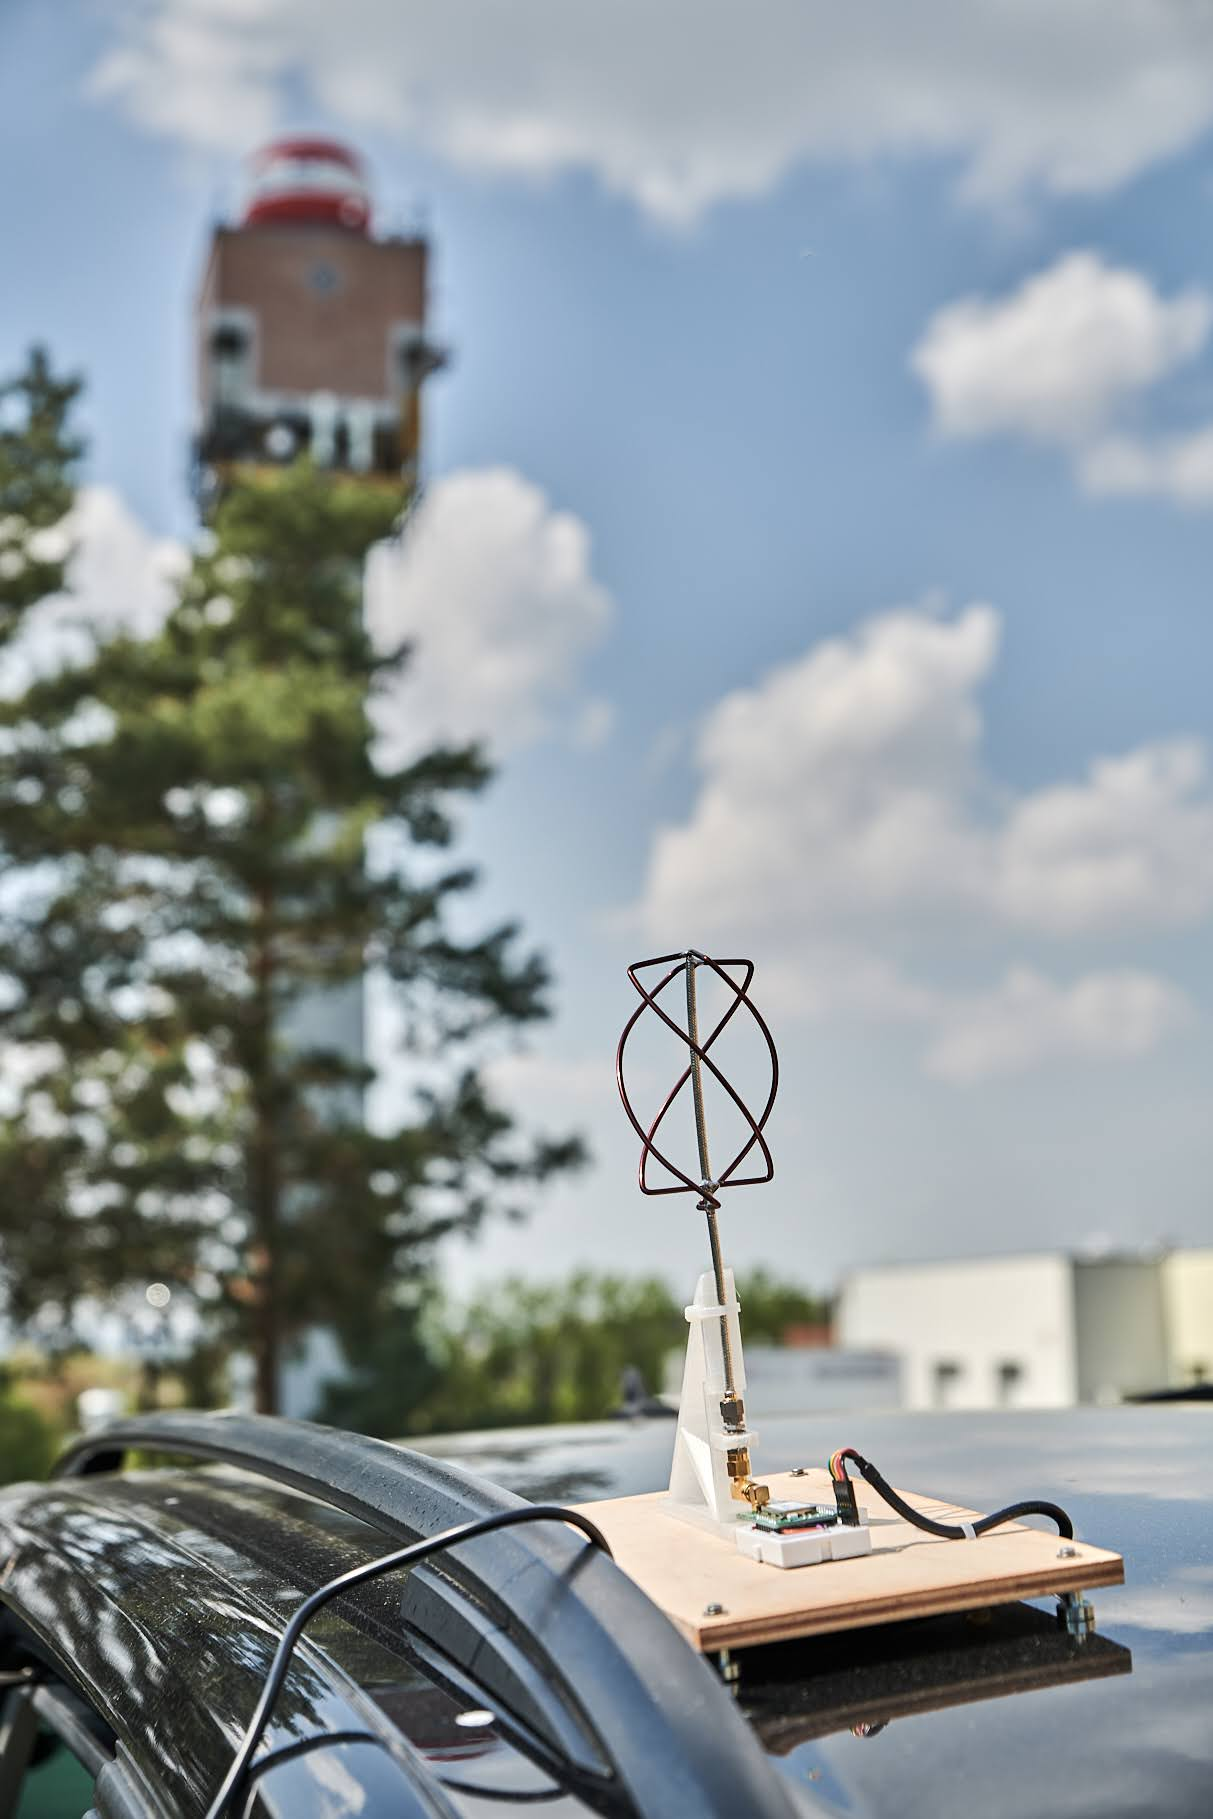
\includegraphics[width=.6\textwidth]{Figures/antena_auto.jpeg}
		\caption{Anténa na příjem dat pro vykreslování pozice na mapě}
		\label{fig:auto:antena}
	\end{figure}


	Zpracování telemetrických údajů pro zobrazení pozice sondy na mapě, výpis výšky sondy a teploty okolí probíhá v Python skriptu. Ten čte skrze sériovou linku data jdoucí z radiopřijímače. Data jsou příjmána do bufferu a následně rozdělena podle dělících znaků viz kód \ref{lst:track:read:parse}.
	\lstinputlisting[language=Python, caption={Blok kódu pro příjem a rozdělení telemetrických údajů}, label={lst:track:read:parse}]{Code/track_read_parse.py}

	Ingormace o poloze jdoucí z GPS senzoru nelze rovnou využít pro zobrazení pozice na mapě. Formát souřadnic, který posílá GPS přijímač, je ve stupních a minutách -- \lstinline|DDMM.MMMMM DDDMM.MMMMM| viz tabulka \ref{tab:gpgll}. Pro zobrazení souřadnic pomocí \textit{gmplot} je nutné souřadnice převést do formátu desetinných stupňů \lstinline|DD.MMMMM DDD.MMMMM|. Tento převod je proveden následovně. První dvě resp. tři číslice ze zeměpisné šířky resp. délky se ponechají a reprezentují \lstinline|DD| resp. \lstinline|DDD| v novém formátu. Zbylé číslo ve formátu \lstinline|MM.MMMMM| se vydělí~60. Výsledek se dosadí za desetinnou tečku. Algoritmus pro převod v jazyce Python je znázorněn v kódu \ref{lst:track:GPS}.

	\lstinputlisting[language=Python, caption={Převod formátu GPS souřadnic}, label={lst:track:GPS}]{Code/track_coordinates.py}

	Zobrazení souřadnic na mapě je provedeno pomocí modulu \textit{gmplot} (https://github.com/gmplot/gmplot). Ukázka kódu \ref{lst:track:main} ukazuje způsob inicializace modulu a zobrazení souřadnic sondy na mapě. Vzniklý soubor \lstinline|my_map.html| lze otevřít v běžném prohlížeči. Vizualizace přijatých GPS souřadnic je na obr. \ref{fig:track:map}.

	\lstinputlisting[language=Python, caption={Příklad zobrazení GPS souřadnic}, label={lst:track:main}]{Code/track_gnd_displ.py}

	\begin{figure}[hbtp]
		\centering
		\includegraphics[width=\textwidth]{Figures/track_map.PNG}
		\caption{Trajektorie letu zobrazena pomocí python skriptu \ref{lst:track:main}}
		\label{fig:track:map}
	\end{figure}










	\section{Testování a měření}
	%měření odběru, energie pro poslání dat
	Před samotným vypuštěním bylo zapotřebí sondu otestovat. Jak spolehlivost elektroniky v nízkých teplotách, tak přenos telemetrických údajů na velkou vzdálenost. Pro korektní zpracování dat bylo také zapotřebí změřit směrovou charakteristiku antén a do jaké míry obal sondy tuto charakteristiku uvlivňuje.

	Ověření funkčnosti sondy při nízkých teplotách bylo provedeno v klimakomoře na katedře technologie. Díky rázovénu schlazení lze do jisté míry simulovat časový průběh teploty okolí, ve kterém se sonda pohybuje. Sonda byla umístěna do klimakomory \ref{fig:sonda:klimakomora} za pokojové teploty a schlazena na -55 °C. Při této teplotě byla následně ponechána xx minut a byla sledována funkčnost elektroniky. Průbeh teploty okolí měřený dvěma senzory umístěnými v sondě je vidět v grafu... . Z grafu je vidět rozdílná tepelná kapacita použitých senzorů teploty. 

	\begin{figure}[hbtp]
		\centering
		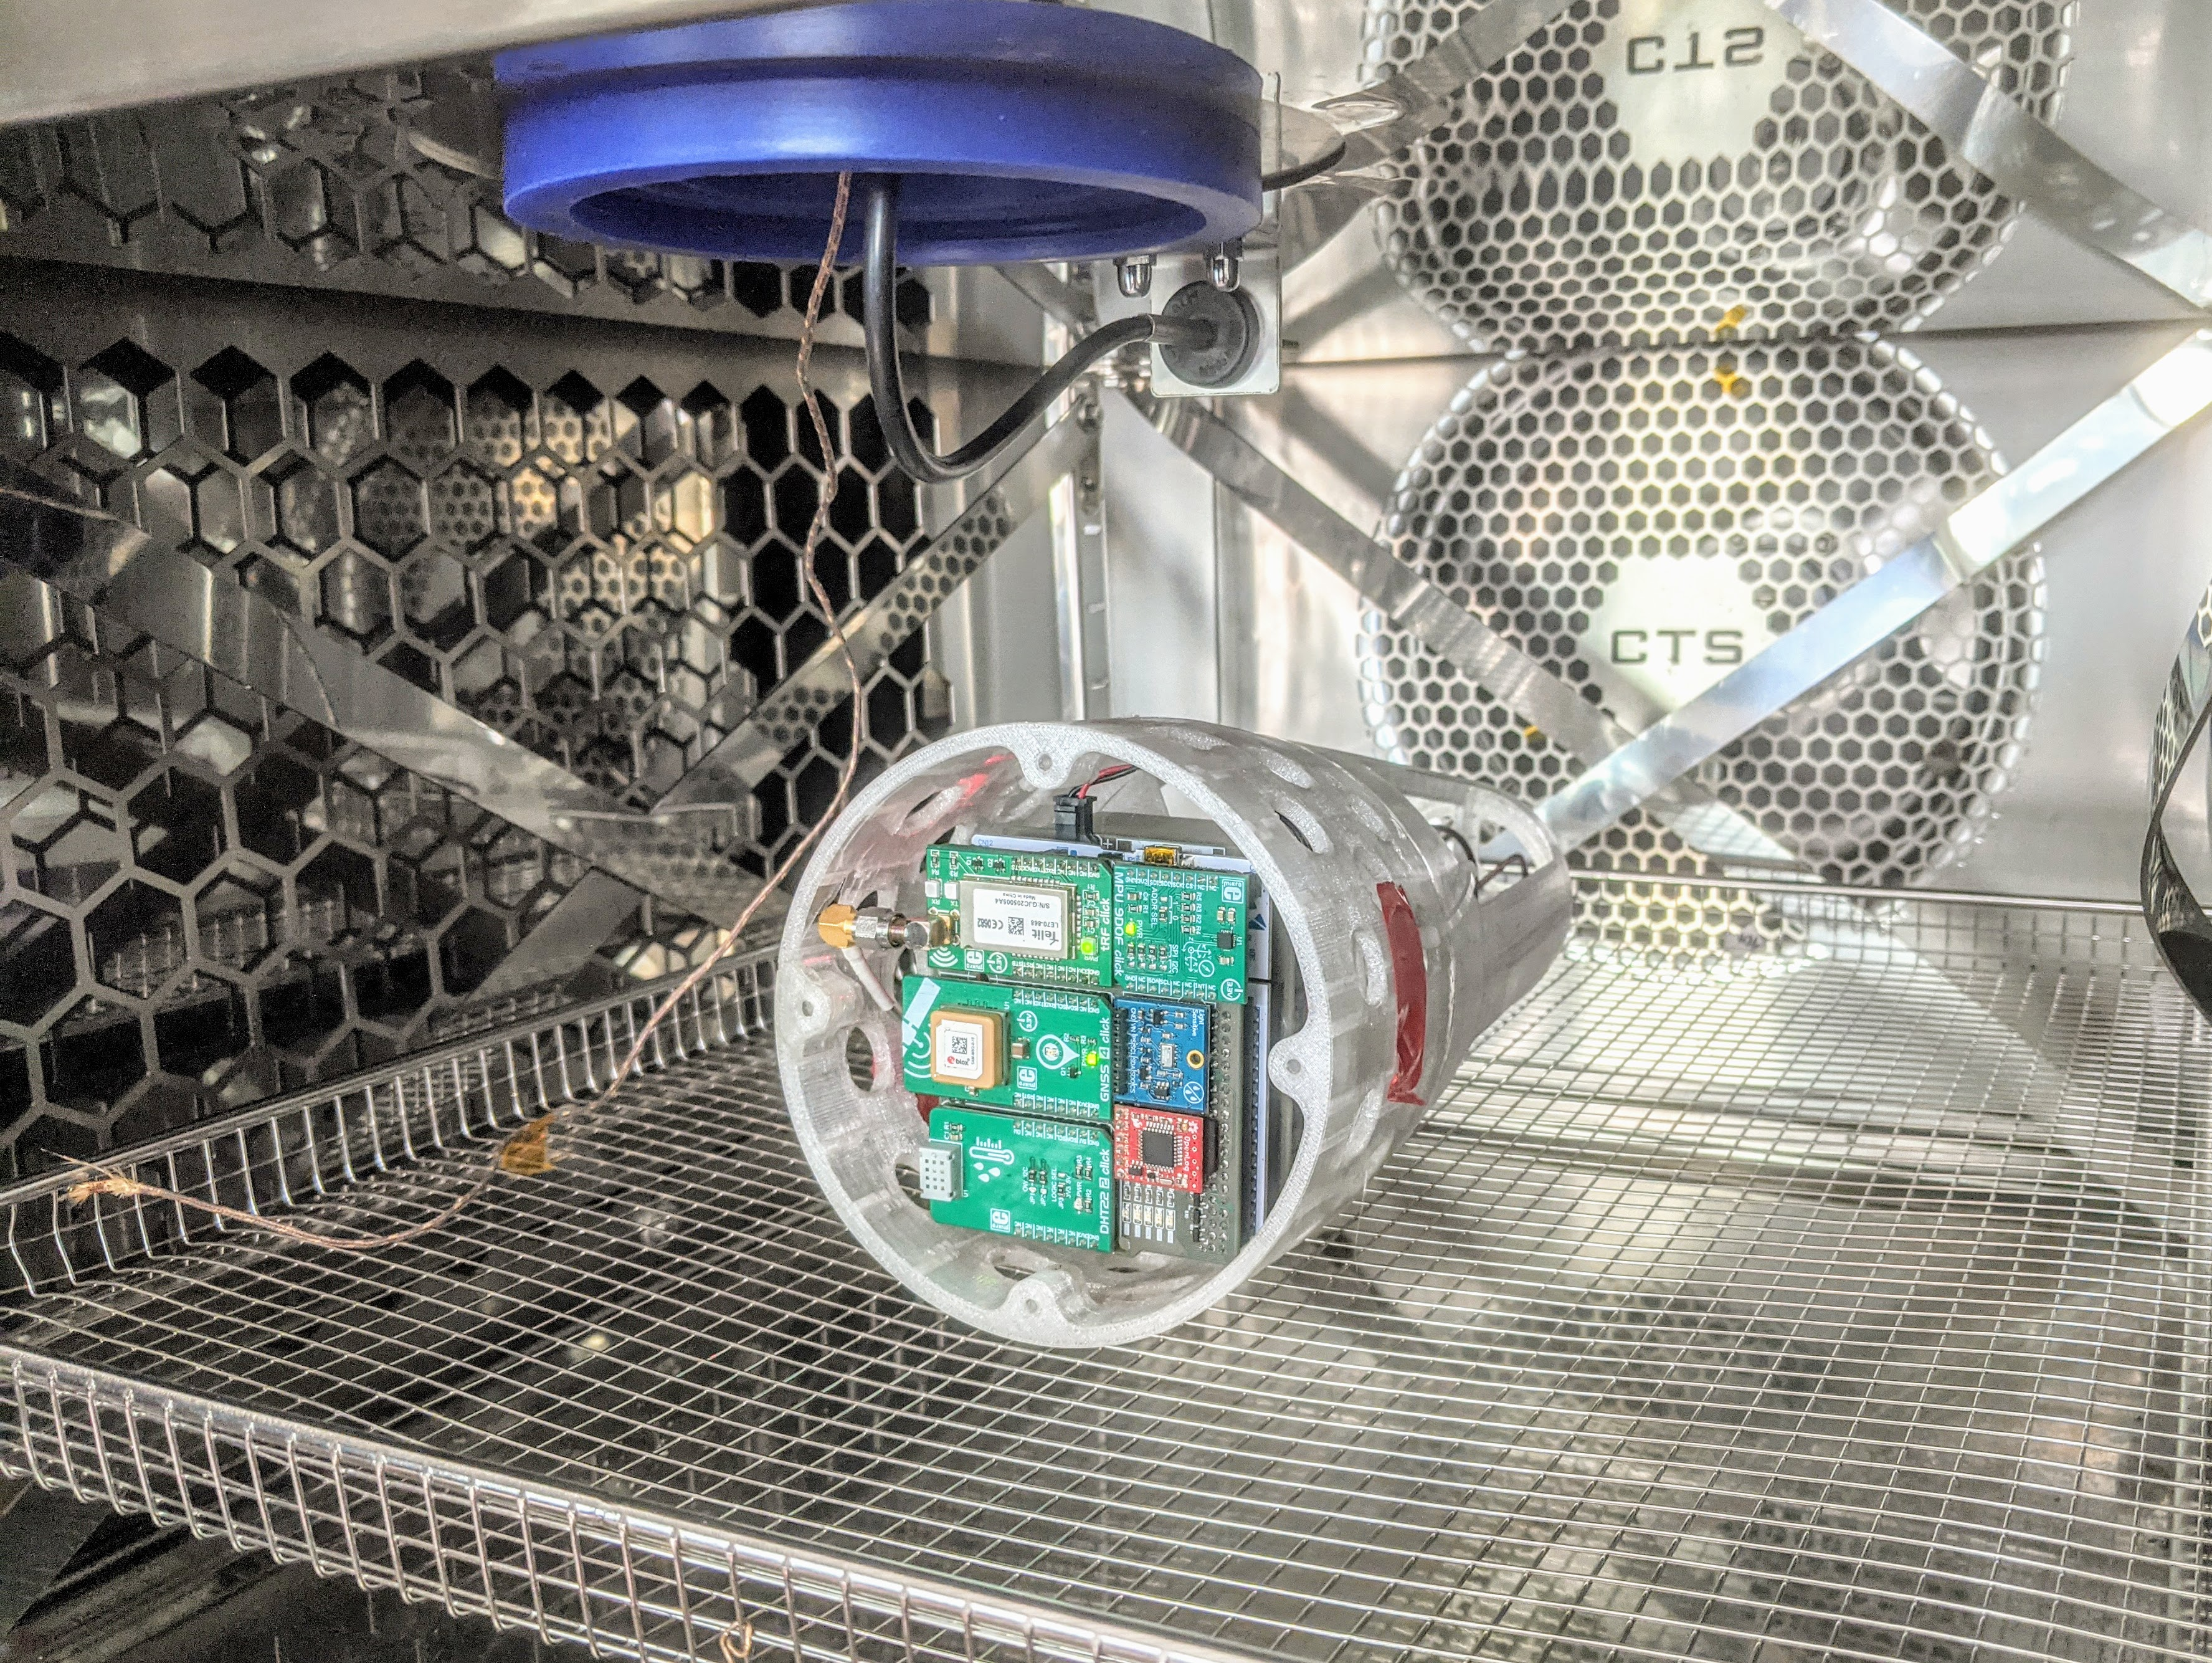
\includegraphics[width=.7\textwidth]{Figures/sonda_klimakomora.jpg}
		\caption{Sonda umístěna v klimakomoře}
		\label{fig:sonda:klimakomora}
	\end{figure}

	TODO: průbeh teploty v klimošce

	Měření směrové charakteristiky proběhlo na katedře elektromagnetického pole v bezodrazné komoře. Sonda připevněna na pohyblivou osu byla otáčena motorem a byl měřen přijatý výkon anténou umístěné naproti sondě. Díky tomu byla změřena vyzařovací charakteristika antény v rozsahu 360~°. Celkem byly měřeny 4 směrové charakteristiky a to pro různá natočení sondy kolem své vlastní osy. Směrové charakteristiky antény jsou zaneseny na obr. \ref{graph:radiation:char}.

	\begin{figure}[hbtp]
		\centering
		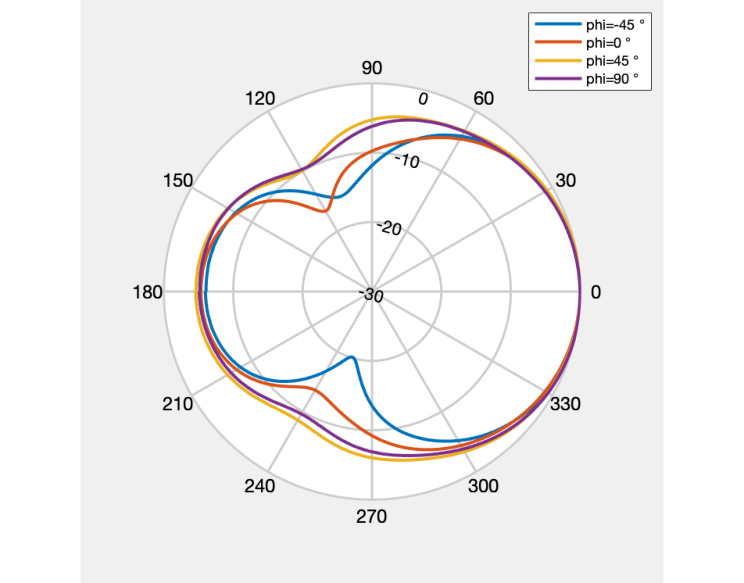
\includegraphics[width=.5\textwidth]{Graphs/radiation_plot.pdf}
		\caption{Směrové charakteristiky antény pro různá natočení kolem její osy}
		\label{graph:radiation:char}
	\end{figure}


	Dále byla měřena polarizace antény. V tomto případě byla sonda pevně umístěna na podstavci a otáčeno bylo přijímací anténou v její ose. Pro ideální kruhově polarizovanou anténu by nezáleželo na natočení přijímací antény. V případně antény umístěné v sondě je přenos znárorněn na obr. xxx.

	TODO - graf polarizace\\
	TODO - spočíst koeficient polarizace, ale je to teď vůbec potřeba? Nebo jen zajímavost?

	Pro ověření dosahu radiového spoje byl přenos dat nejdříve vyzkoušen na zemi. Vysílací část spoje se nacházela na střeše panelévého domu na Petřinách. Přijem probíhal na hoře Říp. Radiový spoj byl realizován na přímou viditelnost a nebyla zakryta 1. Fresnelova zóna, jak je vidět profilu zemského povrchu na obr. \ref{fig:praha:rip}.

	\begin{figure}[hbtp]
		\centering
		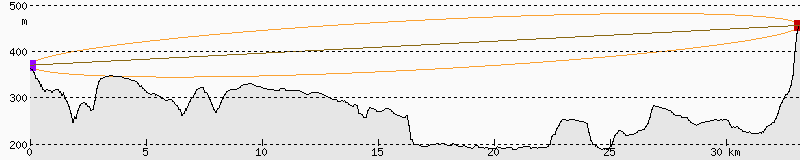
\includegraphics[width=\textwidth]{Figures/petriny_rip.png}
		\caption{Profil trasy mezi Prahou a horou Říp, vykresleno pomocí \url{http://www.heywhatsthat.com/ } }
		\label{fig:praha:rip}
	\end{figure}


%popsat i antenu k modulum
%antenu hodit nahoru a jen napsat, ze jsem j
%anotace 




	

	





























	

	

\chapter{Experiment}
\label{chap:expoeriment}
	V následující kapitole je popsán průběh experimentu od přípravy až po nález sondy. Dále jsou zobrazena surová data ze sondy a ze spektrálního analyzátoru a popsáno jejich čištění, aby bylo možné je dál používat při zpracování. Anténa použitá pro příjem dat byla stejného typu jako na sondě. Umístěna byla na střeše budovy v Dejvicíh na anténním sledovači (obr.~\ref{fig:ground:tracker}), který upravoval orientaci podle polohy cíle - sondy. Ze střechy vedl koaxiální kabel do místnosti, kde byl signál rozbočovačem rozdělen do spektrálního analyzátoru a radiového přijímače v pozemní stanici. Schéma zapojení je zaneseno na obr.~\ref{fig:ground:segment:sch}.
	\begin{figure}[hbtp]
		\centering
		\begin{subfigure}{.49\textwidth}
			\centering
			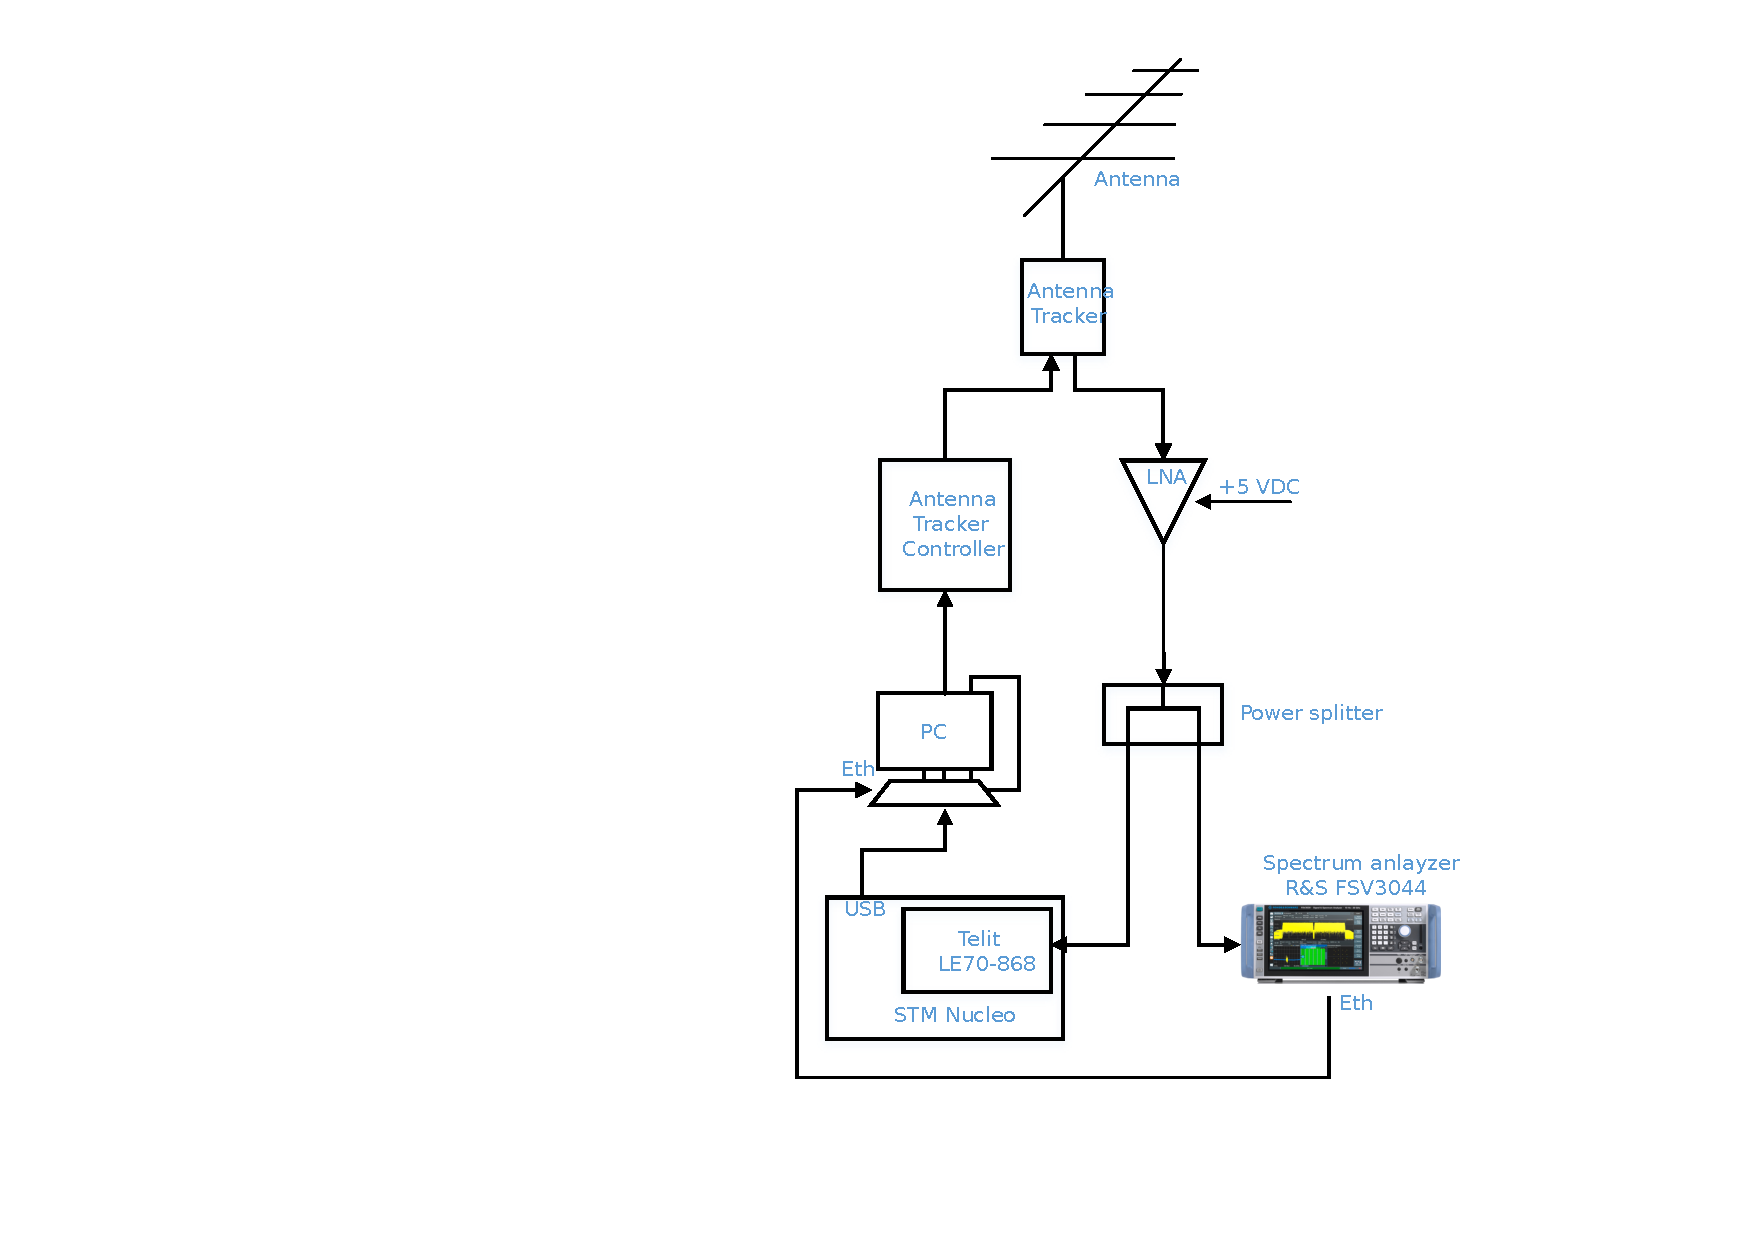
\includegraphics[height=1.2\textwidth]{Figures/ground_segment.pdf}
			\caption{Schéma pozemního segmentu}
			\label{fig:ground:segment:sch}
		\end{subfigure}
		\begin{subfigure}{.49\textwidth}
			\centering
			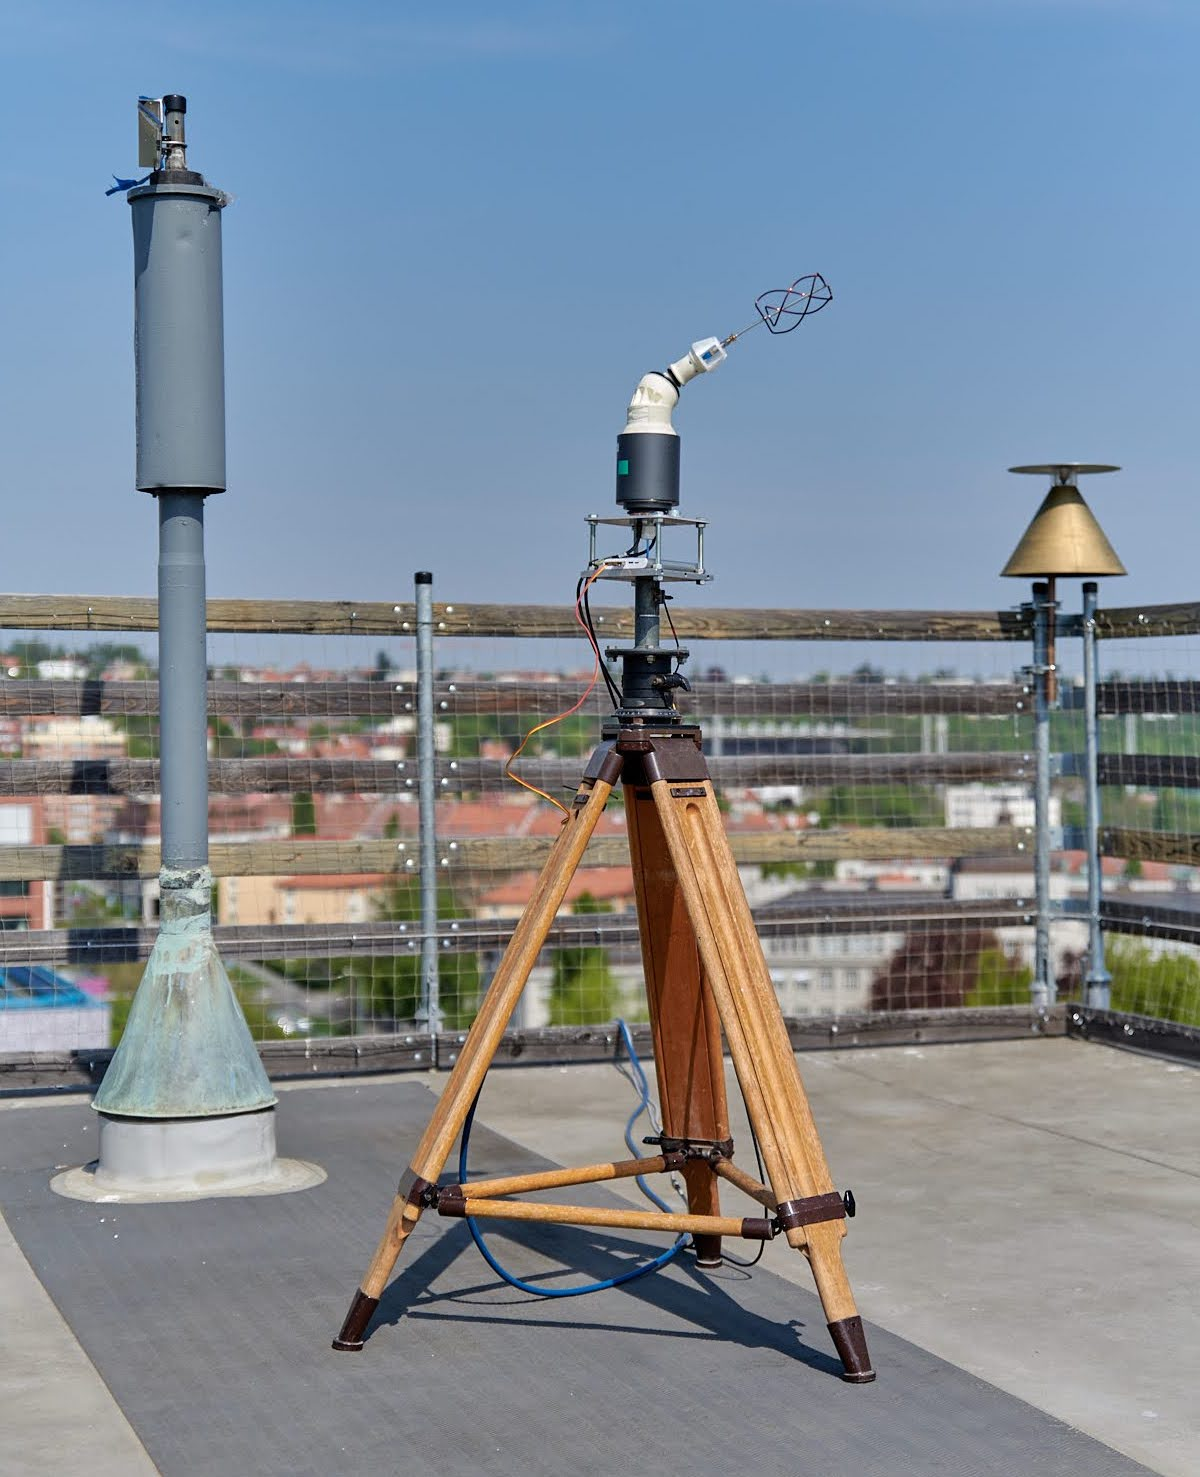
\includegraphics[height=1.2\textwidth]{Figures/tracker.jpg}
			\caption{Anténní sledovač}
			\label{fig:ground:tracker}
		\end{subfigure}
		\caption{Pozemní segment}
		\label{fig:ground}
	\end{figure}



	\section{Průběh experimentu}
	Po přichycení sondy ČHMÚ byla sonda zapnuta a vyčkáno na zjištění GPS pozice. Poté byl pracovníky ústavu napuštěn balón o hmostnosti 1200~g, do kterého byl předem vložen padák. Přesně v 13:15:20 SELČ byl balón se sondami vypuštěn. Ihned po startu byly byly vidět telemetrické údaje o pozici a výšce a byla vykreslována trajektorie letu na mapě. Přibližně po patnácti minutách jsme nasedli do automobilu a vyrazili na místo, kde byl predikován dopad sondy.

	Po 27~minutách letu bylo vysílání telemetrických údajů přerušeno. Podle podledních zaznamenaných údajů se tak stalo v 13:42:53 při teplotě -40~°C v nadmořské výšce 9650.3~m. Sonda již nezačala po dobu letu vysílat. Pozice dopadu byla následně zjištěna podle pozice, kterou vysílala sonda ČHMÚ. Její vysílaná data jsou dekódována radoamatéry a zveřejňována na internetu. Po určení pozice sondy ČHMÚ byla nalezena i má sonda a to o 50~m jihozápadně. Toto bylo dáno 50m provázkem mezi sondami a směrem větru.


	\begin{figure}[hbtp]
		\centering
		\begin{subfigure}{.49\textwidth}
			\centering
			\includegraphics[height=.8\textwidth]{Figures/sonda_strom.jpeg}
			\caption{Sonda visící na stromě}
			\label{fig:sonda:strom}
		\end{subfigure}
		\begin{subfigure}{.49\textwidth}
			\centering
			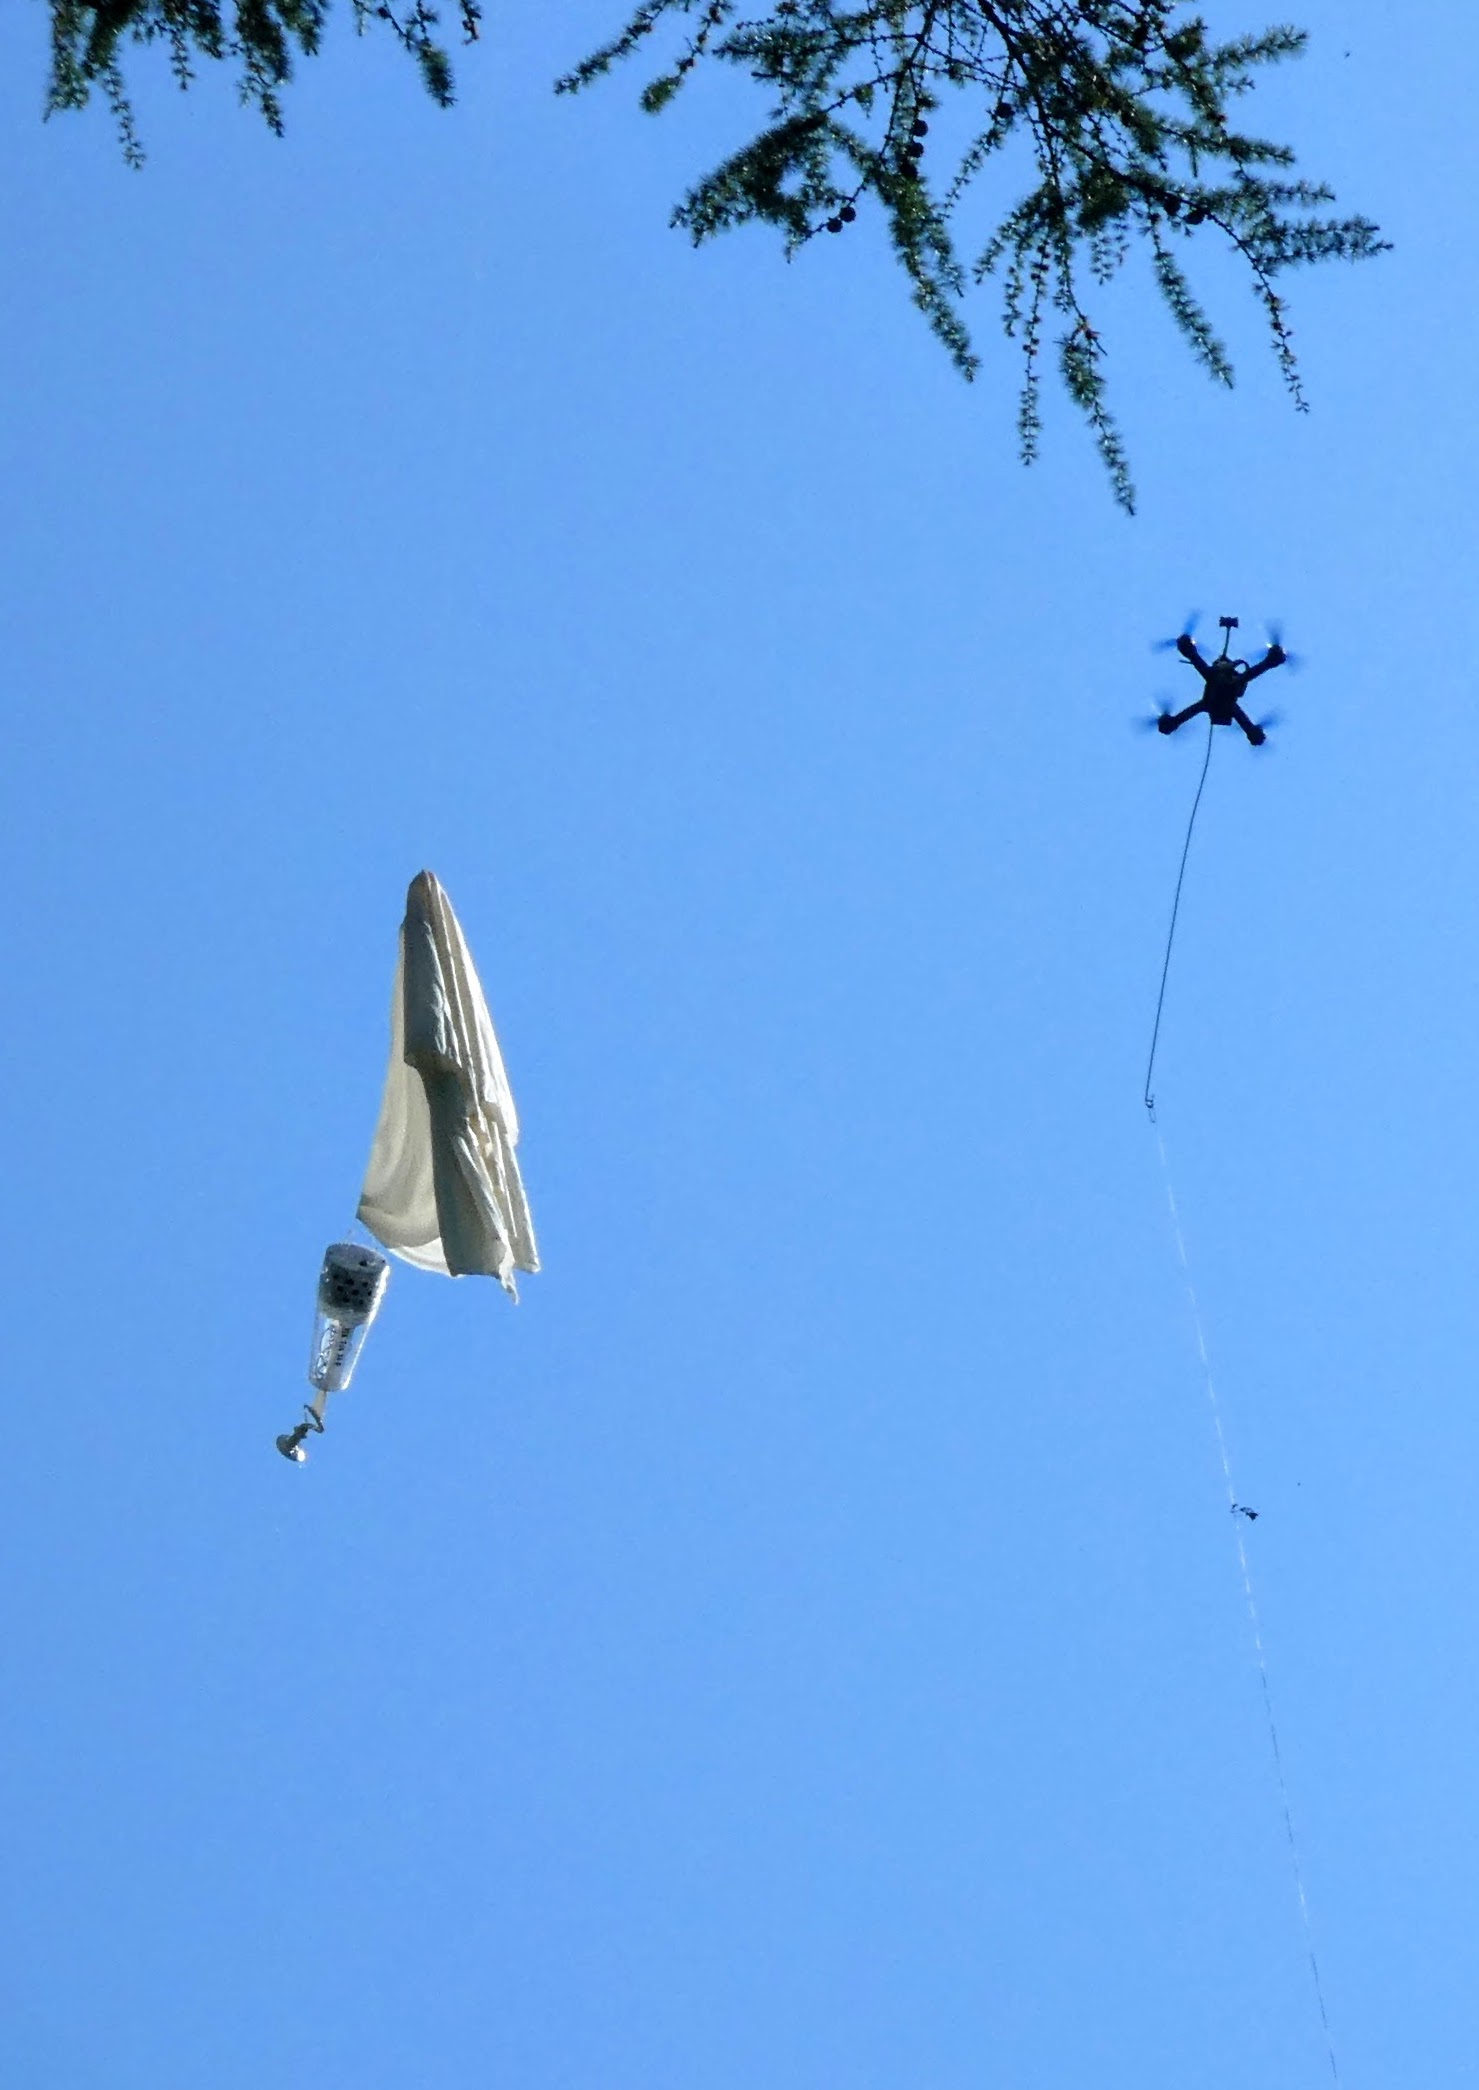
\includegraphics[height=.8\textwidth]{Figures/sonda_dron.jpeg}
			\caption{Sonda a dron použitý k jejímu sundání}
			\label{fig:sonda:dron}			
		\end{subfigure}
	\end{figure}
	


	\section{Naměřená data}
	Jak bylo zmíněno v kapitole o firmwaru sondy, program byl ošetřen několika způsoby, díky kterým se sonda restartovala, pokud nastal nějaký problém. Z dat na SD kartě je patrné, že cyklus čtení dat někdy zachytil příjmanou zprávu z GPS v takové fázi, že neodpovídala předepsanému formátu a tedy nebyla do daných polí uložena odpovídající data. Jestliže se sonda z nějakého důvodu restartuje, inicializace senzorů stvá delší dobu, než je perioda posílání dat. Tedy se může stát, že v momentě, kdy je sonda připravena přijímat GPS data je již GPS přijímač posílá a tedy příjem začne uprostřed posílané zprávy. Příklad chybného formátování dat je např.:
	\begin{center}
		SA\textbf{2512.00}\textbf{5000.34466N01426.89992E}D-002.740066821-03.5;037.9;N;29.868;77
	\end{center}
	Z tučně zvýrazněných dat jsou poznat minuty sekundy a milisekundy a souřadnice sondy.

	Tato data jsou dále nepoužitelna a proto bylo potřeba řádky, které je obsahovaly, odstranit. Odstanění poškozených řádků proběhlo následujícím \textit{UNIX}ovým příkazem provedeným v terminálu, který vybere všechny řádky, obsahující jednu ze dvou následujících posloupností znaků.
	\begin{lstlisting}[language=Awk]
	grep '00;;;;;;;\|00;50' raw_data.txt > data_clean.txt\end{lstlisting}
	Tedy buď nulové milisekundy a prázdná pole o poloze, a nebo nulové milisekundy a první dvě číslice zeměpisné šířky, která se při pohybu sondy s ohledem na dolet nemění. 
	\begin{table}[h!]
		\centering
		\begin{tabular}{l}
			110225.\hl{00;;;;;;;}+029.21;0097759;+28.2;027.7;0;05;4.46;3.46;2.82;8305;-1120;1644;8320;\\
			-7;235;148;-52;10;17;\\\hline
			110226.\hl{00;50}00.41136;N;01426.85498;E;257.1;0.264;+029.20;0097766;+28.3;027.6;1;05;\\
			4.46;3.46;2.82;8304;-1120;1662;8286;3;233;147;-29;14;45;
		\end{tabular}
	\end{table}

	Data ze spektrálního analyzátoru byla ukládána ve formátu \textit{numpy} a obsahovala časovou značku a přijatý výkon. Čas byl ve formátu epoch. Ten udává aktuální čas v sekundách uplynulých od 1. ledna 1970. Například vypuštění v epoch formátu je 1651662920.0000. Tento formát byl převeden po načtení souboru v programu Matlab příkazem
	\begin{lstlisting}[language=Matlab]
		datetime(powerData(:,[1]),'convertfrom', 'posixtime').\end{lstlisting}
	\begin{table}
		\centering
		\begin{tabular}{l|l}
			Čas ve formátu epoch &	Přijatý výkon (dBm)\\\hline
			1651662920.1542&       -77.4421920776\\
			1651662922.1421 &      -78.0411224365\\
			1651662924.1554  &     -84.5278778076\\
			...&...
		\end{tabular}
		\caption{Surová data času a výkonu změřeného spektrálním analyzátorem}
	\end{table}





\chapter{Výsledky}
	Tato kapitola se zabývá zpracováním naměřených dat v programu Matlab. Před samotným zpracováním bylo také potřeba data upravit tak, aby se z nich daly vykreslovat grafy. Například převést časové údaje ukládané s daty na časový formát Matlabu. Díky nim se z dat daly vytvořit časové tabulky \textit{timetable}, které šlo posléze spojit dohromady právě na základě časových údajů u jednotlivých měření. 

	\section{Výstup z experimentu}
	%zkombinovat data ze země a data ze strato, vzorečky, určit refrakci, výkonovou bilanci podle podmínek, vzít v potaz směrovou charstiku. vyrobit model šíření, grafy


	Výpočet refraktivity troposféry byl proveden podle doporučení ITU-R P.453 \cite{ITU:refrac}. Refraktivitu v závoslosti na podmínkách prostředí lze přibližně vyjádřit jako
	\begin{align}
		N = \frac{77.6}{T} \left(P + 4810\frac{e}{T}\right),
		\label{eq:refr:meas}
	\end{align}
	kde $T$ je absolutní hodnota v K, $p$ je atmosférický tlak v hPa a $e$ je tlak vodních par v hPa. Ten lze vypočíst pomocí hustoty vodních par z doporučení ITU-R 836 \cite{ITU:vapour}. Pdle \cite{ITU:refrac} lze tlak vodních par vypočítat také podle relativní vlhkosti vzduchu $H$ jako
	\begin{align}
		e = \frac{H}{100}\,6{,}1121\,\mt{e}^{\frac{17{,}502t}{240{,}97 + t}},
	\end{align}
	kde $t$ je teplota v °C. Vztah platí v rozsahu teplot od -20 °C do 50 °C \cite{zaklady:sireni:vln}.

	Pro aproximaci výškového profilu rekraktivity ITU doporučuje \cite{ITU:refrac} exponenciální model podle vztahu:
	\begin{align}
		N = N_\mt{0}\,\mt{e}^{-h/h_\mt{0}},
		\label{eq:refr:approx}
	\end{align}
	kde $h$ je výška nad zemí, $N_\mt{0}$ hodnota refraktivity v 0~km a $h_\mt{0}$ výškové měřítko v km. ITU udává globální světový průměr $N_\mt{0} = 315 \mt{ N}$ a $h_\text{0} = 7{,}35 \mt{ km}$ \cite{zaklady:sireni:vln}.
	\begin{figure}[hbtp]
		\centering
		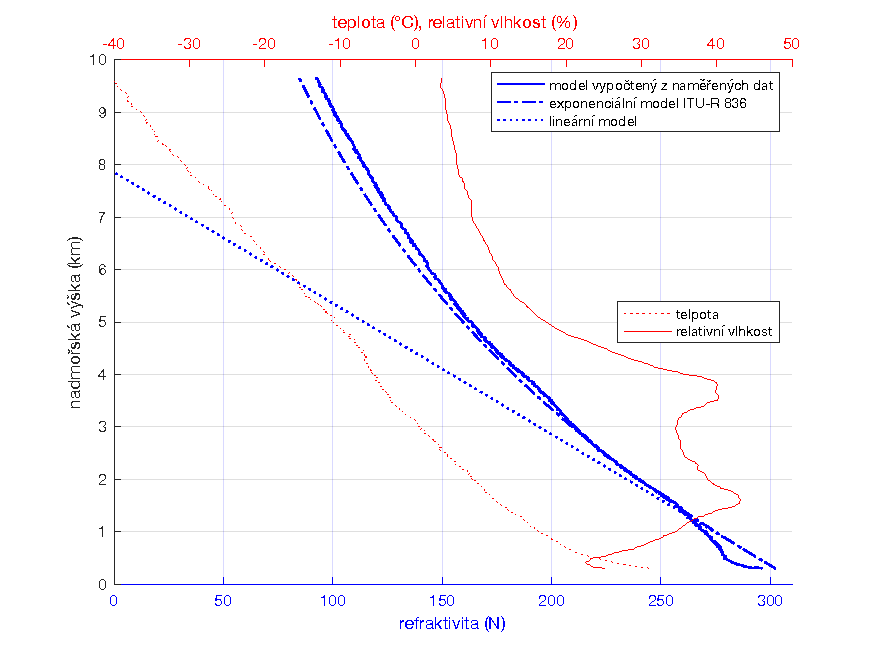
\includegraphics[width=.7\textwidth]{Graphs/refractivity_exp_lin_meas_hum.pdf}
		\caption{Výškový profil refraktivity}
		\label{graph:refr}
	\end{figure}

	Data refraktivity vypočtené pomocí \eqref{eq:refr:meas} byla proložena exponenciální funkcí viz obr.~\ref{graph:refr:fit}. Výpočet koeficientů byl proveden pomocí funkce v Matlabu \lstinline[language=Matlab]|fit(alt,N,'exp1');|, kde \lstinline|alt| je vektor nadmořských výšek v metrech a \lstinline|N| je vektor vypočtených refraktivit pro dané nadmořské výšky.

	Výsledná proložená funkce ve tvaru $y=a\,\mt{exp}(b\,x)$ vyšla jako
	\begin{align}
		N(h) = 304{,}7\,\mt{e}^{-0{,}000123\,h}.
		\label{eq:exp:fit}
	\end{align}
	Z naměřených dat vychází hodnota refraktivity v 0~km jako $N_\mt{0} = 304{,}7 \mt{ N}$. Porovnáním exponentů z \eqref{eq:refr:approx} a \eqref{eq:exp:fit} dostaneme
	\begin{align}
		\begin{split}
		-h/h_\mt{0} &= -0{,}000123\,h\\
		h_\mt{0} &= 1/0{,}000123 \mt{ (m)}\\
		h_\mt{0} &= 8130{,}1 \mt{ m}.
		\end{split}
	\end{align}
	Hodnota výškového měřítka vyšla z proložení dat $h_\mt{0} = 8{,}13 \mt{ km}$.
	\begin{figure}[hbtp]
		\centering
		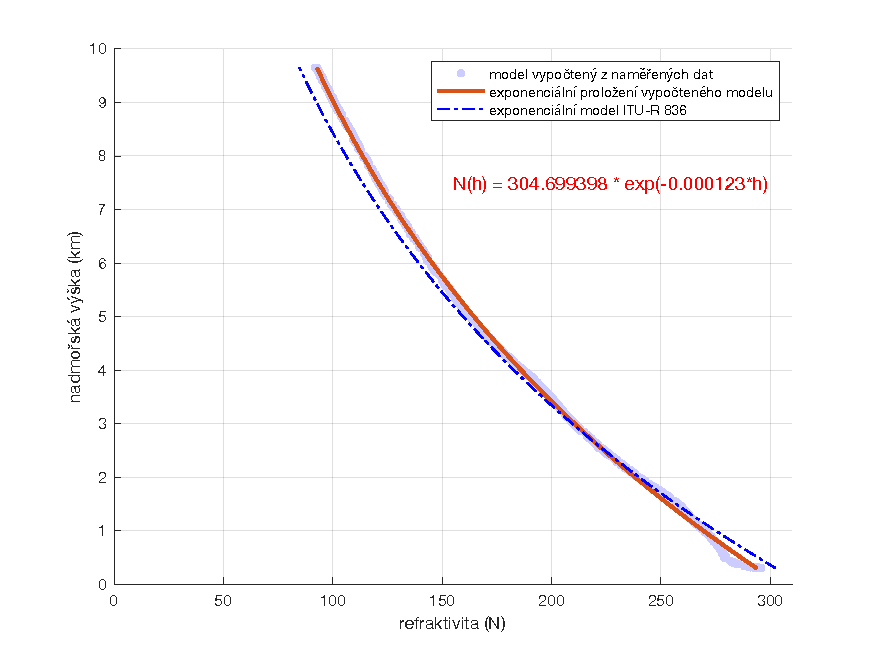
\includegraphics[width=.7\textwidth]{Graphs/refractivity_meas_fit_model.pdf}
		\caption{Proložené hodnoty refraktivity exponenciální křivkou}
		\label{graph:refr:fit}
	\end{figure}

	\begin{figure}
		\centering
		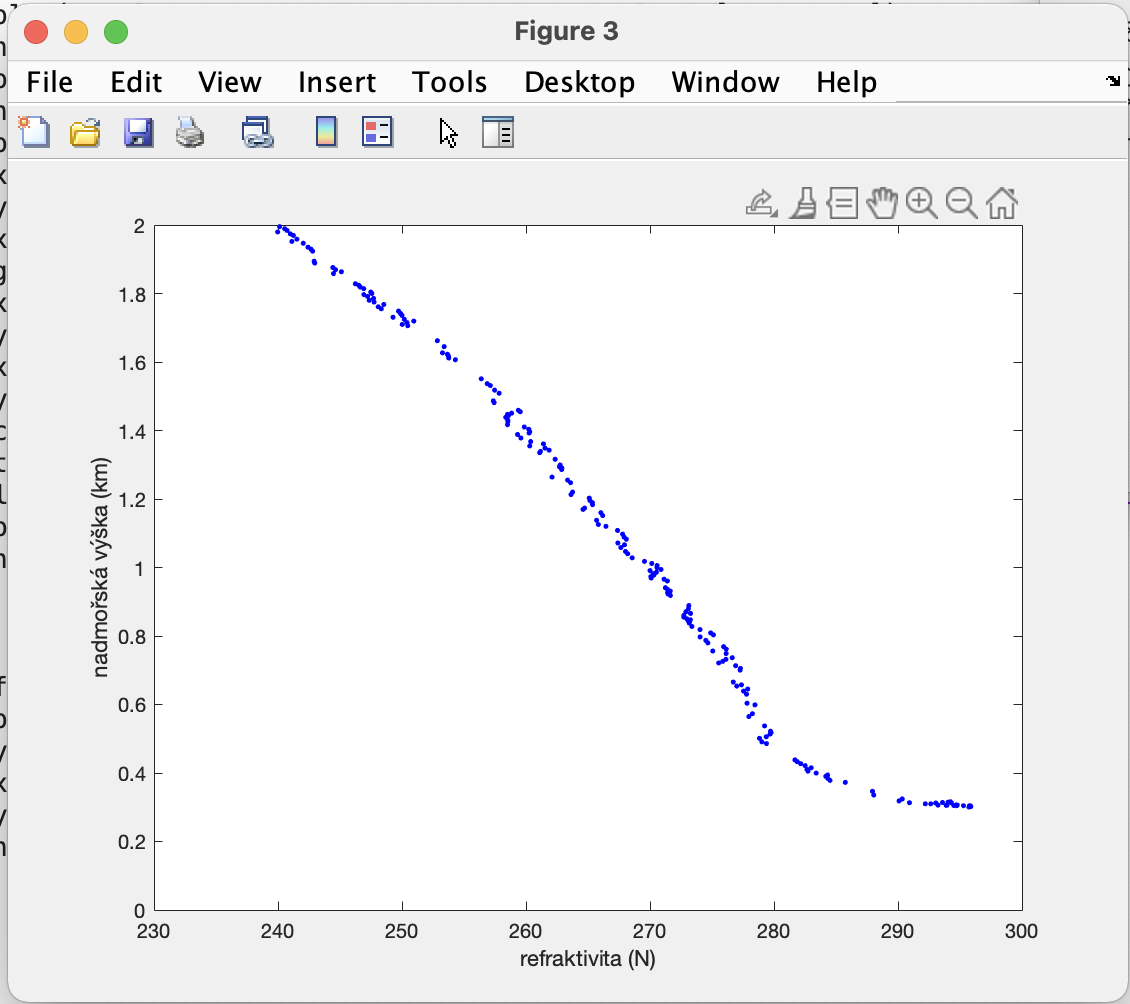
\includegraphics[width=.7\textwidth]{Graphs/ref2km.png}
		\caption{Profil refraktivity pro první dva kilometry}
		\label{graf:refr:2km}
	\end{figure}

	Data o přijatém výkonu anténou bohužel nelze použít. Jak bylo po dokončení experimentu zjištěno, při komunikaci anténního sledovače a jeho řídicí jednotky došlo k rušení a přijímací anténa se začala nepředvídatelně natáčet. Toto je vidět na obr.~\ref{grah:p:alt:hum}, kdy zcela bez jakýhkoliv výrazných změn okolního prostředí došlo k prudkémnu poklesu signálu. Šlo o moment, kdy se anténa vlivem rušení v komunikaci natočila jiným směrem, než byla sonda. Bohužel vinou tohoto chování sledovače není možné data použít k ověření ztrát způsobenými šířením ve volném prostoru a ztrá způsobenými refraktivitou atmosféry. 

	\begin{figure}[hbtp]
		\centering
		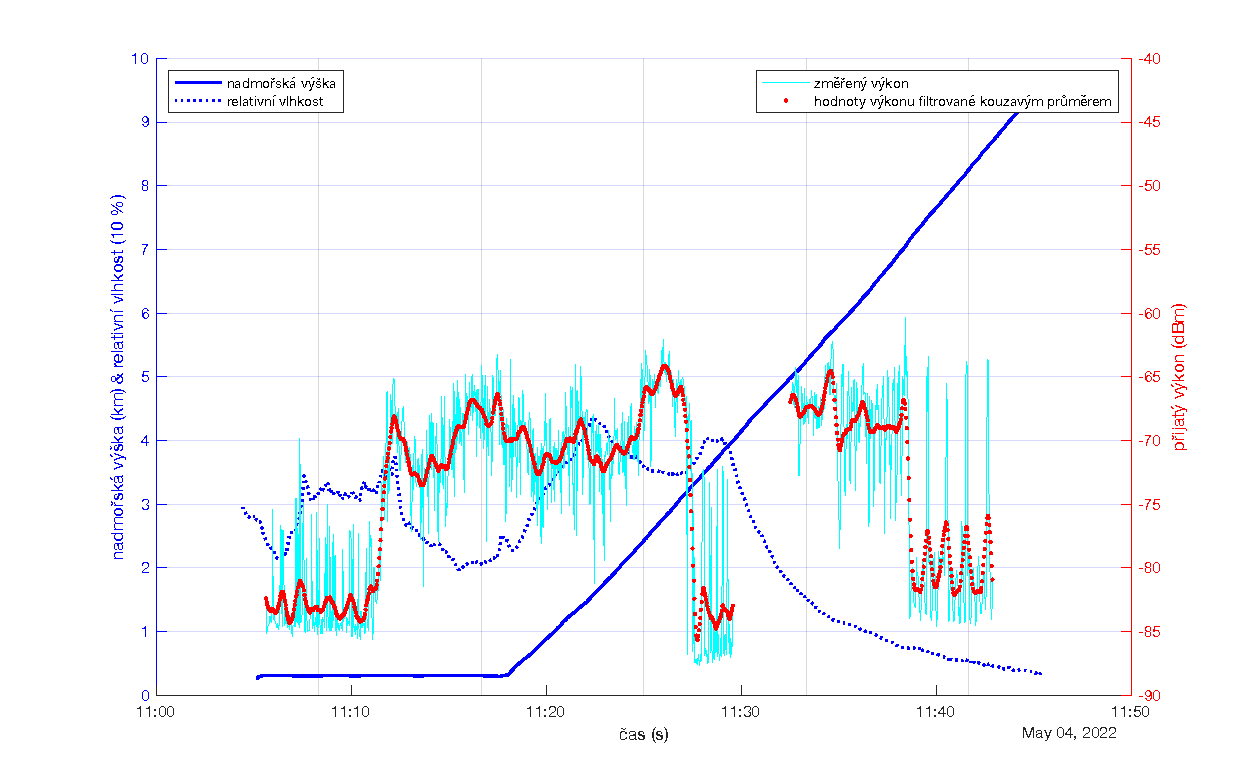
\includegraphics[width=.9\textwidth]{Graphs/alt_hum_p_p_filt.pdf}
		\caption{Průběh výkonu přijatého spektrometrem, výšky sondy a vlhkosti okolí v čase}
		\label{grah:p:alt:hum}
	\end{figure}

	Jelikož v tomto případě není přijatý výkon téměř vůbec závislý na vzdálenosti sondy a pozemního segmentu, nebudou takto data ani interpretována. 

	TODO:POLOMĚR OHYBU V ZÁVISLOSTI NA REFRAKTIVITĚ poloměr na str. 79
	TODO:do grafu hodit závislot FLS na vzdálenosti (má to vůbec smysl?)

















	


\chapter{Závěr}
	\section{Shrnutí experimentu}
	%co se povedlo, co se nepovedlo. Vyrobil jsem sondu a sw, přestala vysílat - proč? 
	V rámci práce vznikla sonda schopná měřit podmínky ve stratosféře a vybraná data posílat na zem. Bylo zařízeno její vypuštění pod záštitou ČHMÚ a po dopadu byla sonda opět nalezena. Dále vzniky podpůrné jednotky určené pro příjem dat ze sondy a jejich zpracování v reálném čase.

	I přes testování sondy v nízkých teplotách, panujících ve vyšších vrstvách zemské atmosféry, bylo posílání a zapiování dat zastaveno. Nicméně naměřená data do 10~km stačila pro vytvoření modelu šíření radiového signálu.

	Anténní sledovač, použitý pro sledování sondy ze střechy FEL v Dejvicích bohužel znehodnotil měřená data. Vinou rušení mezi řídicím boxem a elektronikou zodpovědnou za otáčení antény, došlo k náhodným otáčením antény a příjem signálu v nespecifikovaném bodě směrové charakteristiky. 

	Data naměřena sondou byla využita při tvorbě výškového gradientu refraktivity a ten byl porovnán s doporučeným exponenciálním modelem podle \cite{ITU:refrac}. Koeficienty doporučeného modelu byly porovnány s koeficienty exponenciálního proložení modelu vznikým v rámci této práce. 



	\section{Možná vylepšení}
	%malé DPS bez modulů, optimalizace sw, nepoužívat HAL, programovat přes registry, měření náklonu sondy, častější posílání dat, nezávislost na GPS.
	Hlavním problémem po elektronické stránce bylo využití senzorů ve formě modulů a ne jako čipů samotných. Nemožnost zkrátit zbytečné dlouhé napájecí přívody k čipům a dlouhé komunikační cesty mohly mít za následek celkovou nefunkčnost sondy. Jsou to nicméně problémy, keré se mohou objevit jen za velmi specifických podmínek a testování je nemusí odhalit. V dalším vývoji je proto zcela logické již dělat samotné DPS, které bude obsahovat všechny komponenty potřebné pro správné fungování sondy.

	Software byl založen na HAL knihovnách od firmy \textit{STMicroelectronics}. Ty jsou dobré pro jednoduché programy, nicméně jejich omezená dokumetace znemožňuje tvorbu bezpečného kódu. Psaní kódu na úrovni registrů je tedy jedna z cest, jak zajistit bezpečný kód s předvídatelným chováním. Takový kód nicméně vyžaduje hlubší povědomí o programování mikroprocesorů.

	Pro přesné určení bodu, kterým anténa směřovala na pozemní segment je potřeba kombinace dat z akcelerometru, gyroskopu a magnetometru. Byla zmíněna metoda \textit{Kalmánova filtru}. Díky tomu by se nemuselo počítat s typickým rozkmitem, ale v daný moment relativně přesně určit směřování sondy. \textit{Kalmánův filtr} se běžne využívá napřáklad v dronech a některé řídící algorytmy mají otevřený kód, který lze použít pro inspiraci.

	Jak je kód napsán, spoléhá na přicházející data z GPS přijímače a každou sekundu s jejich příchodem provede odečtení dat, jejich zpracování a poslání a uložení na SD kartu. V případě, že odpojíme GPS přijímač, nebudou odečítány žádné hodnoty. Zlepšení vidím v nezávislosti posílání dat na GPS přijímači.

	Jako poslední místo na zlepšení vidím vyřazení dosavadního anténního sledovače z pozemního segmentu a využití všesměrové antény s fixním úchytem.

	Všechna tato vylepšení mají své místo v další revizi sondy a jednotek kolem ní. Jsou ideálním začtkem při navazování na tuto práci ať už autorem a nebo nadšeným čtenářem.
	
















	


\appendix

\printindex

\appendix
\begin{thebibliography}{1}
	\bibitem{zaklady:sireni:vln}PECHAČ, Pavel a Stanislav ZVÁNOVEC. \textit{Základy šíření vln pro plánování pozemních rádiových spojů}. Praha: BEN - technická literatura, 2007. ISBN 978-80-7300-223-7.

	\bibitem{web_tropo}\textit{Atmospheric Structure} [online] \url{https://www.albany.edu/faculty/rgk/atm101/structur.htm} [cit.~2022-05-19]

	\bibitem{ITU:vapour}ITU-R Rec. P.836, \textit{Water vapour: surface density and total columnar content}, Geneva, [online] \url{https://www.itu.int/dms_pubrec/itu-r/rec/p/R-REC-P.836-6-201712-I!!PDF-E.pdf} [cit.~2022-05-19]

	\bibitem{ITU:refrac}ITU-R Rec. P.453, \textit{The radio refractive index: its formula and refractivity data}, Geneva, [online] \url{https://www.itu.int/dms_pubrec/itu-r/rec/p/R-REC-P.453-14-201908-I!!PDF-E.pdf} [cit.~2022-05-19]

	\bibitem{AOE}HOROWITZ, Paul a Winfield HILL. \textit{The art of electronics}. Third edition. New York: Cambridge University Press, 2015. ISBN 978-0-521-80926-9.

	\bibitem{web_sledovani}\textit{Tracking a Weather Balloon}
    \url{https://www.highaltitudescience.com/pages/tracking-a-weather-balloon} [cit.~2022-05-19]

	\bibitem{web_ctu}\textit{Vyhláška o technických a provozních podmínkách amatérské radiokomunikační služby}, [online] \url{https://www.zakonyprolidi.cz/cs/2005-156#cast1} [cit.~2022-05-19]

	\bibitem{web_spot}\textit{Spot Trace User Guide}
    \url{https://www.findmespot.com/downloads/SPOT_TRACE_User_Guide.pdf} [cit.~2022-05-19]

	\bibitem{dsh_lmr}\textit{LMR33630 Datasheet}\url{https://www.ti.com/lit/ds/symlink/lmr33630.pdf?ts=1652260993140&ref_url=https%253A%252F%252Fwww.google.com%252F} [cit.~2022-05-19]

	\bibitem{dsh_gps}\textit{U-Blox SAM-M8Q Datasheet}\url{https://content.u-blox.com/sites/default/files/SAM-M8Q_DataSheet_%28UBX-16012619%29.pdf} [cit.~2022-05-19]

	\bibitem{dsh_mpu_map}\textit{MPU9250 Register Map}\url{https://invensense.tdk.com/wp-content/uploads/2015/02/RM-MPU-9250A-00-v1.6.pdf} [cit.~2022-05-19]

	\bibitem{dsh_mpu}\textit{MPU9250 Datasheet}\url{https://invensense.tdk.com/wp-content/uploads/2015/02/PS-MPU-9250A-01-v1.1.pdf} [cit.~2022-05-19]

	\bibitem{dsh_AM2320}\textit{AM2320 Datasheet}\url{https://cdn-shop.adafruit.com/product-files/3721/AM2320.pdf} [cit.~2022-05-19]

	\bibitem{dsh_MS5607}\textit{MS5607 Datasheet}\url{https://www.te.com/commerce/DocumentDelivery/DDEController?Action=showdoc&DocId=Data+Sheet%7FMS5607-02BA03%7FB2%7Fpdf%7FEnglish%7FENG_DS_MS5607-02BA03_B2.pdf%7FCAT-BLPS0035} [cit.~2022-05-19]

	\bibitem{dsh_ldo}\textit{LDO 1117-3v3 Datasheet}\url{https://www.st.com/resource/en/datasheet/ld1117.pdf} [cit.~2022-05-19]

	\bibitem{dsh_AA}\textit{Energizer ultimate lithium Datasheet}\url{https://data.energizer.com/pdfs/l92.pdf} [cit.~2022-05-19]

	\bibitem{vaisala_foto}\textit{Nun ein wenig Information zu der Sonde RS41-SG
	}\url{https://www.qsl.net/oe1ffs/Sondenpage/RS41/RS41.html} [cit.~2022-05-19]

	\bibitem{dsh_vaisala}\textit{Vaisala RS41 Datasheet}\url{https://www.vaisala.com/sites/default/files/documents/WEA-MET-RS41SGP-Datasheet-B211444EN.pdf} [cit.~2022-05-19]

	%\bibitem{dsh_}\textit{Datasheet}\url{} [cit.~2022-05-19]



\end{thebibliography}
%\bibliographystyle{amsalpha}
%\bibliography{bibb}

\ctutemplate{specification.as.chapter}

\end{document}

%vaisala datasheet https://www.vaisala.com/sites/default/files/documents/WEA-MET-RS41SGP-Datasheet-B211444EN.pdf